
%--------------------------------------------------------------------------
%
%  M.Sc. Thesis
%  By: Mohammad Raziei
%
%--------------------------------------------------------------------------

%--------------------------------------------------------------------------
%
%  LaTeX Thesis Template (v2.2)
%  By: Hamid Zarrabi-Zadeh
%
%  Contributors:
%      Ehsan Emamjomeh-Zadeh
%      Omid Gheibi
%
%--------------------------------------------------------------------------


\documentclass[oneside,a4paper,12pt,table]{book}
%\usepackage[bottom]{footmisc}
%\usepackage{stfloats}
%\fnbelowfloat % puts footnotes below the bottom floats
%\makeatletter
%\renewcommand{\fps@figure}{htp}
%\renewcommand{\fps@table}{htp}
%\makeatother
\toks0{\ifvoid\footins\else\suppressfloats[b]\fi} 
\output\expandafter{\the\toks0\the\output}

%\usepackage{minipage-marginpar}

\usepackage[inline]{enumitem}
\newlist{alphinline}{enumerate*}{1}
\setlist[alphinline]{label=(\alph*)}
\newlist{enuminline}{enumerate*}{1}
\setlist[enuminline]{label=(\arabic*)}
\newlist{circlelist}{enumerate}{1}
\setlist[circlelist,1]{label=\protect\circled{\arabic*}}
\newlist{alphabetlist}{enumerate}{1}
\setlist[alphabetlist]{label=\alph*)}
\newlist{checklist}{itemize}{1}
\setlist[checklist]{label=$\checkmark$)}
\newlist{iteminline}{itemize*}{1}
\setlist[iteminline]{label=$\bullet$}

\usepackage{placeins}
\usepackage{comment}
\usepackage{etoolbox}
\newcounter{magicrownumbers}
\usepackage{tabularx, longtable}
\usepackage{ltablex}

\usepackage{currfile-abspath}

%%%%%%%%%%%%%%%%%%%%%
\usepackage{pdftexcmds}
\makeatletter
\newcommand{\stringcases}[3]{%
	\romannumeral
	\str@case{#1}#2{#1}{#3}\q@stop
}
\newcommand{\str@case}[3]{%
	\ifnum\pdf@strcmp{\unexpanded{#1}}{\unexpanded{#2}}=\z@
	\expandafter\@firstoftwo
	\else
	\expandafter\@secondoftwo
	\fi
	{\str@case@end{#3}}
	{\str@case{#1}}%
}
\newcommand{\str@case@end}{}
\long\def\str@case@end#1#2\q@stop{\z@#1}
\makeatother

%%%%%%%%%%%%%%%%5


%\newcommand*{\dothis}[1]{%
%	\stringcases
%	{#1}%
%	{%
%		{a}{so you typed a}%
%		{b}{now this is b}%
%		{c}{you want me to do c?}%
%	}%
%	{[nada]}%
%}


\usepackage{siunitx}
\usepackage{catchfile}

\newcommand*\readNumFromFile[2][\num]{%
	\CatchFileDef{\tempnum}{#2}{}%
	#1{\tempnum}%
}



\usepackage{booktabs,longtable}
\usepackage{adjustbox}
\usepackage{csvsimple} % For csv importing.

\makeatletter
\csvset{
	autotabularcenter/.style={
	file=#1,
	after head=\csv@pretable\begin{tabular}{|*{\csv@columncount}{c|}}\csv@tablehead,
	table head=\hline\csvlinetotablerow\\\hline,
	late after line=\\,
	table foot=\\\hline,
	late after last line=\csv@tablefoot\end{tabular}\csv@posttable,
	command=\csvlinetotablerow},
}
\makeatother
\makeatletter
\csvset{
	autotabularcentercolorheader/.style={
		file=#1,
		after head=\csv@pretable\begin{tabular}{|*{\csv@columncount}{c|}}\csv@tablehead,
			table head=\hline\rowcolor{headerColor}\csvlinetotablerow\\\hline,
			late after line=\\,
			table foot=\\\hline,
			late after last line=\csv@tablefoot\end{tabular}\csv@posttable,
		command=\csvlinetotablerow},
}
\makeatother

\newcommand{\csvautotabularcenter}[2][]{\csvloop{autotabularcenter={#2},#1}}
\newcommand{\csvstyleread}[3][]{\csvloop{#2={#3},#1}}

%\newcommand*{\readcsv}[3][]{%
%	\stringcases{#1}{
%		{a}{\csvloop{autotabularcenter={#3},#2}}%
%	}%
%	{[nada]}
%}
\newcommand*{\readcsv}[2]{%
	\stringcases
	{#1}%
	{%
		{default}{\readfromcsvs{autotabularcenter}{#2}}%
		{simplecenter}{\csvstyleread{autotabularcenter}{#2}}%	
		{centercolorheader}{\csvstyleread{autotabularcentercolorheader}{#2}}%
		{b}{now this is b}%
		{c}{you want me to do c?}%
	}%
	{[nada]}%
}



\usepackage{listings, color}
\definecolor{dkgreen}{rgb}{0,0.6,0}
\definecolor{gray}{rgb}{0.5,0.5,0.5}
\definecolor{lightgray}{rgb}{0.8,0.8,0.8}
\definecolor{mauve}{rgb}{0.58,0,0.82}

\lstset{frame=tBLr,
	%	frameround=fttt,
	language=Matlab,
	aboveskip=3mm,
	belowskip=3mm,
	showstringspaces=false,
	columns=flexible,
	basicstyle={\small\ttfamily},
	lineskip=0.5em,
	xleftmargin=23pt,
	xrightmargin=9pt,
	framexleftmargin=17pt,
	framexrightmargin=5pt,
	framexbottommargin=2pt,
	numbers=left,
	firstnumber=1,
	numberstyle=\tiny\color{gray},
	keywordstyle=\color{blue},
	commentstyle=\color{dkgreen},
	stringstyle=\color{mauve},
	rulecolor=\color{black},
	breaklines=true,
	breakatwhitespace=true,
	tabsize=4
}


% -------------------------------------------------------
%  Common Styles and Formattings
% -------------------------------------------------------

\usepackage[table, svgnames, dvipsnames]{xcolor}
\usepackage{color}


\usepackage{amsthm, thmtools}
\usepackage{environ}
%\usepackage{bickham}
%\usepackage{boondox-cal}
%\usepackage{boondox-calo}
\usepackage{dutchcal}
\usepackage{amssymb,amsmath,gensymb,mathtools}
\usepackage{pxfonts}
\usepackage{stackengine}


\usepackage[hyphens]{url}%\PassOptionsToPackage{hyphens}{url}
\usepackage[colorlinks,linkcolor=blue,citecolor=blue, breaklinks]{hyperref}
\usepackage{xurl}
%\usepackage{url}


%\usepackage{breakurl}
\usepackage{copyrightbox,doi}
\usepackage[usenames,dvipsnames]{pstricks}
\usepackage{graphicx,subfigure,wrapfig}
\usepackage[bottom]{footmisc}
\usepackage{geometry,fancyhdr}
\usepackage[mathscr]{euscript}
\usepackage[version=4]{mhchem}

\usepackage{tabularx,multirow,multicol,array}
\newcolumntype{C}[1]{>{\centering\arraybackslash\hspace{0pt}}p{#1}}
\newcolumntype{Y}{>{\centering\arraybackslash}X}
\definecolor{headerColor}{rgb}{0.78,0.85,.95}

\usepackage{algorithmicx,algorithm}



\usepackage{placeins}
\usepackage{comment}
\usepackage{etoolbox}
\newcounter{magicrownumbers}
\usepackage{tabularx, longtable}
\usepackage{ltablex}

%======================================================================================

\usepackage[inline]{enumitem}
\newlist{alphinline}{enumerate*}{1}
\setlist[alphinline]{label=(\alph*)}
\newlist{enuminline}{enumerate*}{1}
\setlist[enuminline]{label=(\arabic*)}
\newlist{circlelist}{enumerate}{1}
\setlist[circlelist,1]{label=\protect\circled{\arabic*}}
\newlist{alphabetlist}{enumerate}{1}
\setlist[alphabetlist]{label=\alph*)}
\newlist{checklist}{itemize}{1}
\setlist[checklist]{label=$\checkmark$)}
\newlist{iteminline}{itemize*}{1}
\setlist[iteminline]{label=$\bullet$}

%--------------------------------------------------------------------------------------
\usepackage{makeidx}\makeindex
\usepackage[localise=on,extrafootnotefeatures]{xepersian} %%%%%%%%%%%%%%%%%%%%%%%%%%%
\usepackage[noend]{algpseudocode}


%------------------------ Algorithm ------------------------------------

\newenvironment{الگوریتم}[1]
	{\bigskip\bigskip\begin{algorithm}\caption{#1} \label{الگوریتم: #1}\vspace{0.5em}\begin{algorithmic}[1]}
	{\end{algorithmic}\vspace{0.5em}\end{algorithm}\bigskip}
	

\renewcommand{\algorithmicfor}{{به ازای}}
\renewcommand{\algorithmicwhile}{{تا وقتی}}
\renewcommand{\algorithmicdo}{\hspace{-.2em}:}
\renewcommand{\algorithmicif}{{اگر}}
\renewcommand{\algorithmicthen}{\hspace{-.2em}:}
\renewcommand{\algorithmicelse}{{در غیر این صورت:}}
%\renewcommand{\algorithmicelsif}{{در غیر این صورت اگر: }}
\renewcommand{\algorithmicreturn}{{برگردان}}
\renewcommand{\algorithmiccomment}[1]{$\triangleleft$ \emph{#1}}
\renewcommand{\algorithmicrequire}{\textbf{ورودی:}}
\renewcommand{\algorithmicensure}{\textbf{خروجی:}}

\newcommand{\اگر}{\If}
\newcommand{\وگرنه}{\Else}
\newcommand{\وگر}{\ElsIf}
\newcommand{\پایان‌اگر}{\EndIf}
\newcommand{\به‌ازای}{\For}
\newcommand{\پایان‌به‌ازای}{\EndFor}
\newcommand{\تاوقتی}{\While}
\newcommand{\پایان‌تاوقتی}{\EndWhile}
\newcommand{\دستور}{\State}
\newcommand{\دستورک}{\Statex}
\newcommand{\توضیحات}{\Comment}
\newcommand{\برگردان}{\Return}
\renewcommand{\ورودی}{\Require}
\newcommand{\خروجی}{\Ensure}


\usepackage{bidihl}
\definecolor{lightYellow}{rgb}{1,1,0.73}
\newcommand{\hl}[1]{\bidihl{#1}}
\definecolor{bidihlcolor}{rgb}{1,1,0.73}



%\sethlcolor{yellow}
%\def\SOUL@hlpreamble{%
%	\setul{\dp\strutbox}{\dimexpr\ht\strutbox+\dp\strutbox\relax}%
%	\let\SOUL@stcolor\SOUL@hlcolor
%	\SOUL@stpreamble
%}
%\makeatother
%
%\newcommand{\hlfa}[1]{\hl{\rl{#1}}}
%\newcommand{\hlc}[2][yellow]{\sethlcolor{#2}\hl{#1}}




% -------------------- Page Layout --------------------


\newgeometry{top=3.5cm,bottom=3.5cm,left=2.5cm,right=3cm,headheight=25pt}

\renewcommand{\baselinestretch}{1.4}
\linespread{1.6}
\setlength{\parskip}{0.45em}
%\setlength{\abovedisplayskip}{0pt}
%\setlength{\belowdisplayskip}{0pt}
%\setlength{\abovedisplayshortskip}{0pt}
%\setlength{\belowdisplayshortskip}{0pt}


\fancyhf{}
\rhead{\leftmark}
\lhead{\thepage}

\def\negspace{-2em}
\newcommand{\removevspace}[1][2]{\vspace{-#1em}}
\newenvironment{equationx}{\removevspace$\begin{aligned}}{\end{aligned}$}

% -------------------- Fonts --------------------

\settextfont[
Scale=1.09,
Extension=.ttf, 
Path=styles/fonts/,
BoldFont=XB NiloofarBd,
ItalicFont=XB NiloofarIt,
BoldItalicFont=XB NiloofarBdIt
]{XB Niloofar}

%\setdigitfont[
%Scale=1.09,
%Extension=.ttf, 
%Path=styles/fonts/,
%BoldFont=XB NiloofarBd,
%ItalicFont=XB NiloofarIt,
%BoldItalicFont=XB NiloofarBdIt
%]{XB Niloofar}
\setdigitfont{Yas}

\defpersianfont\sayeh[
Scale=1,
Path=styles/fonts/
]{XB Kayhan Pook}


% -------------------- Styles --------------------


\SepMark{-}
\renewcommand{\labelitemi}{$\small\bullet$}



% -------------------- Environments --------------------


\newtheorem{قضیه}{قضیه‌ی}[chapter]
\newtheorem{لم}[قضیه]{لم}
\newtheorem{ادعا}[قضیه]{ادعای}
\newtheorem{مشاهده}[قضیه]{مشاهده‌ی}
\newtheorem{نتیجه}[قضیه]{نتیجه‌ی}
\newtheorem{مسئله}{مسئله‌ی}[chapter]
\newtheorem{تعریف}{تعریف}[chapter]
\newtheorem{مثال}{مثال}[chapter]


\newenvironment{اثبات}
	{\begin{trivlist}\item[\hskip\labelsep{\em اثبات.}]}
	{\leavevmode\unskip\nobreak\quad\hspace*{\fill}{\ensuremath{{\square}}}\end{trivlist}}

\newenvironment{alg}[2]
	{\begin{latin}\settextfont[Scale=1.0]{Times New Roman}
	\begin{algorithm}[t]\caption{#1}\label{algo:#2}\vspace{0.2em}\begin{algorithmic}[1]}
	{\end{algorithmic}\vspace{0.2em}\end{algorithm}\end{latin}}




%\newtheorem*{note}{توجه}

\newtheoremstyle{notethm}% 
{}{}% 
{\itshape}{}% 
{}{}% 
{ }% 
{\colorbox{headerColor}
	{\textbf{\thmname{#1}\thmnumber{ #2}}
		\thmnote{ (#3)}.}}

\declaretheorem[style=notethm,title=\rl{توجه}]{note}
%\def\createmyenvironment#1#2#3{\declaretheorem[style=#1,title=#3]{#2}}
%\createmyenvironment{notethm, note, \rl{توجه}}


% -------------------- Titles --------------------


\renewcommand{\listfigurename}{فهرست شکل‌ها}
\renewcommand{\listtablename}{فهرست جدول‌ها}
\renewcommand{\bibname}{\rl{{مراجع}\hfill}} 


% -------------------- Commands --------------------


\newcommand{\IN}{\ensuremath{\mathbb{N}}} 
\newcommand{\IZ}{\ensuremath{\mathbb{Z}}} 
\newcommand{\IQ}{\ensuremath{\mathbb{Q}}} 
\newcommand{\IR}{\ensuremath{\mathbb{R}}} 
\newcommand{\IC}{\ensuremath{\mathbb{C}}} 

\newcommand{\set}[1]{\left\{ #1 \right\}}
\newcommand{\seq}[1]{\left< #1 \right>}
\newcommand{\ceil}[1]{\left\lceil{#1}\right\rceil}
\newcommand{\floor}[1]{\left\lfloor{#1}\right\rfloor}
\newcommand{\card}[1]{\left|{#1}\right|}
\newcommand{\setcomp}[1]{\overline{#1}}
\newcommand{\provided}{\,:\,}
\newcommand{\divs}{\mid}
\newcommand{\ndivs}{\nmid}
\newcommand{\iequiv}[1]{\,\overset{#1}{\equiv}\,}
\newcommand{\imod}[1]{\allowbreak\mkern5mu(#1\,\,\text{پیمانه‌ی})}

\newcommand{\poly}{\mathop{\mathrm{poly}}}
\newcommand{\polylog}{\mathop{\mathrm{polylog}}}
\newcommand{\eps}{\varepsilon}

\newcommand{\lee}{\leqslant}
\newcommand{\gee}{\geqslant}
\renewcommand{\leq}{\lee}
\renewcommand{\le}{\lee}
\renewcommand{\geq}{\gee}
\renewcommand{\ge}{\gee}

\newcommand{\مهم}[1]{\textbf{#1}}
\renewcommand{\برچسب}{\label}

\newcommand{\REM}[1]{}
\renewcommand{\حذف}{\REM}
\newcommand{\لر}{\lr}
\newcommand{\کد}[1]{\lr{\tt #1}}
\newcommand{\پاورقی}[1]{\footnote{\lr{#1}}}

\newcommand{\urlSource}[1]{\lr{\scriptsize{source: \url{#1}}}}
\newcommand{\doiSource}[1]{\lr{\scriptsize{source: \doi{#1}}}}

\newcommand{\hcenter}[1]{\makebox[\textwidth][c]{#1}}

\newcommand{\Doi}[1]{\lr{\doi{#1}}}



\AtBeginEnvironment{figure}{\setcounter{subfigure}{0}}% Resets subfigure counter at start of figure environment

%.cwl
\NewEnviron{copyrightBox}[3][b]{
	%	\setcounter{subfigure}{0}% Reset subfigure counter
	\noindent\copyrightbox[#1]{
		\begin{minipage}{#2}\BODY\end{minipage}
	}{#3}}
%.cwl
\NewEnviron{RTLcopyrightBox}[3][b]{
	%	\setcounter{subfigure}{0}% Reset subfigure counter
	\noindent\copyrightbox[#1]{
		\begin{minipage}{#2}
			\begin{RTL}	\BODY \end{RTL}
		\end{minipage}
	}{#3}}

% -------------------- Dictionary --------------------


\newcommand{\dicalphabet}[1]{
\begin{minipage}{\columnwidth}
	\centerline{\noindent\textbf{\large #1 }}
	\vspace{.5em}
\end{minipage}
\nopagebreak[4]
}

\newcommand{\dic}[2]{\noindent  #2 \dotfill  \lr{#1} \\ }


% ------------------------------ Images and Figures --------------------------

\graphicspath{{figs/}}
\setlength{\intextsep}{0pt}  % for float boxes
\renewcommand{\psscalebox}[1]{}  % for LaTeX Draw

\newcommand{\floatbox}[2]
	{\begin{wrapfigure}{l}{#1}
	\centering #2 \end{wrapfigure}}

\newcommand{\centerfig}[2]
	{\centering\scalebox{#2}{\input{figs/#1}}}

\newcommand{\fig}[3]
	{\floatbox{#3}{\centerfig{#1}{#2}}}

\newcommand{\centerimg}[2]
	{\vspace{1em}\begin{center}\includegraphics[width=#2]{figs/#1}\end{center}\vspace{-1.5em}}

\NewDocumentCommand{\img}{m m o}
	{\begin{wrapfigure}{l}{\IfValueTF{#3}{#3}{#2}}
	\centering\includegraphics[width=#2]{figs/#1}\end{wrapfigure}}

\newcommand{\f}[2]{$\frac{#1}{#2}$}
\newcommand{\rltext}[1]{\text{\rl{#1}}}
\newcommand{\lrtext}[1]{\text{\lr{#1}}}



\newcommand*{\Scale}[2][4]{\scalebox{#1}{$#2$}}%
\newcommand*{\Resize}[2]{\resizebox{#1}{!}{$#2$}}%
\newcommand\rescaleequation[2]{\resizebox{#1\hsize}{!}{$#2$}}


% -------------------------------------------------------
%  Custom Definitions
% -------------------------------------------------------


\newcommand{\OPT}{\ensuremath{\mathop{\mathrm{OPT}}}}
\newcommand{\APX}{\ensuremath{\mathop{\mathrm{APX}}}}
\newcommand{\ALG}{\ensuremath{\mathop{\mathrm{ALG}}}}


\usepackage[]{ptext}

\newcommand\rownumber{\stepcounter{magicrownumbers}\arabic{magicrownumbers}}
\newcommand\resetrownumber{\preto\tabular{\setcounter{magicrownumbers}{0}}}

\newcommand{\seecode}[2]{\href{#2}{\texttt{#1}}}
\newcommand{\seemycode}[2]{\seecode{#1}{\thepwd../Code/#2}}
\newcommand{\Seemycode}[1]{\seemycode{#1}{#1}}

\renewcommand{\chaptername}{بخش}
%\renewcommand{\thechapter}{\tartibi{chapter}}

\newcommand{\hcenter}[1]{\makebox[\textwidth][c]{#1}}

\graphicspath{ {../Code/results/} }

\newcommand{\urlSource}[1]{\lr{\scriptsize{source: \url{#1}}}}
\newcommand{\doiSource}[1]{\lr{\scriptsize{source: \doi{#1}}}}
\newcommand{\Doi}[1]{\lr{\doi{#1}}}
\newcommand{\mri}{\lr{ MRI}}
\newcommand{\mr}{\lr{ MR}}
\newcommand{\nmr}{\lr{ NMR}}
\newcommand{\kspace}{\lr{ k-space}}
\newcommand{\f}[2]{$\frac{#1}{#2}$}
\newcommand{\rltext}[1]{\text{\rl{#1}}}
\newcommand{\lrtext}[1]{\text{\lr{#1}}}
%\newcommand{\xLeftrightarrow}[2][]{\ext@arrow 0099\Leftrightarrowfill@{#1}{#2}}
\newcommand{\Rho}{\mathcal{P}}
\newcommand{\F}{\mathcal{F}}



\begin{document}
%\setlength{\abovedisplayskip}{0pt}
%\setlength{\belowdisplayskip}{0pt}
%\setlength{\abovedisplayshortskip}{0pt}
%\setlength{\belowdisplay\shortskip}{0pt}

% -------------------- Front Pages --------------------

%\pagenumbering{alph}


% -------------------------------------------------------
%  Thesis Information
% -------------------------------------------------------

\newcommand{\ThesisType}
{پایان‌نامه‌ی کارشناسی ارشد}
\newcommand{\ThesisTitle}
{قالب استاندارد برای نگارش پایان‌نامه‌ها}
\newcommand{\ThesisAuthor}
{حمید ضرابی‌زاده}
\newcommand{\ThesisSupervisor}
{استاد راهنمای پروژه}
\newcommand{\ThesisAdvisor}
{استاد مشاور}
\newcommand{\ThesisExaminer}
{استاد ممتحن}
\newcommand{\ThesisDate}
{شهریور ۱۳۹۹}
\newcommand{\ThesisDepartment}
{دانشکده‌ی مهندسی کامپیوتر}
\newcommand{\ThesisMajor}
{مهندسی نرم‌افزار}
\newcommand{\ThesisUniversity}
{دانشگاه صنعتی شریف}


% -------------------------------------------------------
%  English Information
% -------------------------------------------------------

\newcommand{\EnglishThesisType}{M.Sc. Thesis}

\newcommand{\EnglishThesisTitle}{A Standard Template for Typesetting Theses in Persian}

\newcommand{\EnglishThesisAuthor}{Hamid Zarrabi-Zadeh}

\newcommand{\EnglishThesisSupervisor}{Dr. Supervisor}

\newcommand{\EnglishThesisDate}{September 2020}

\newcommand{\EnglishThesisDepartment}{Department of Computer Engineering}

\newcommand{\EnglishThesisUniversity}{Sharif University of Technology}


\pagestyle{empty}

\begin{center}


\includegraphics[scale=0.2]{front/template/images/logo.png}

\begin{large}

\vspace{-0.2cm}
\ThesisUniversity \\[-0.3em]
مهندسی برق

\vspace{0.5cm}

\ThesisType \\[-0.3em]
مهندسی پزشکی

\end{large}

\vspace{1cm}

{عنوان:}\\[1.2em]
{\LARGE\textbf{کاهش نرخ نمونه برداری \mri}}

\vspace{1cm}

{نگارش:}\\[.5em]
{\large\textbf{محمد رضیئی فیجانی}}

\vspace{0.7cm}

{استاد راهنما:}\\[.5em]
{\large\textbf{دکتر بیژن وثوقی وحدت}}

\vspace{1.3cm}

\ThesisDate

\end{center}

\newpage



\pagestyle{empty}

\begin{center}


\includegraphics[scale=0.75]{front/template/images/besmellah.jpg}

\end{center}

\newpage


% Uncomment the following line for adding signature page
%\input{front/template/signatures.tex}

%\input{front/acknowledge.tex}
%\input{front/abstract.tex}


% -------------------- Table of Contents --------------------


\pagestyle{fancy}

\tableofcontents \newpage
\listoffigures \newpage
\listoftables \newpage

%\pagenumbering{arabic}

% -------------------- Chapters --------------------

%\include{chapters/guide}
%\include{chapters/writing}
%\section{مقدمه}




\begin{figure}[t!]
	\centering
	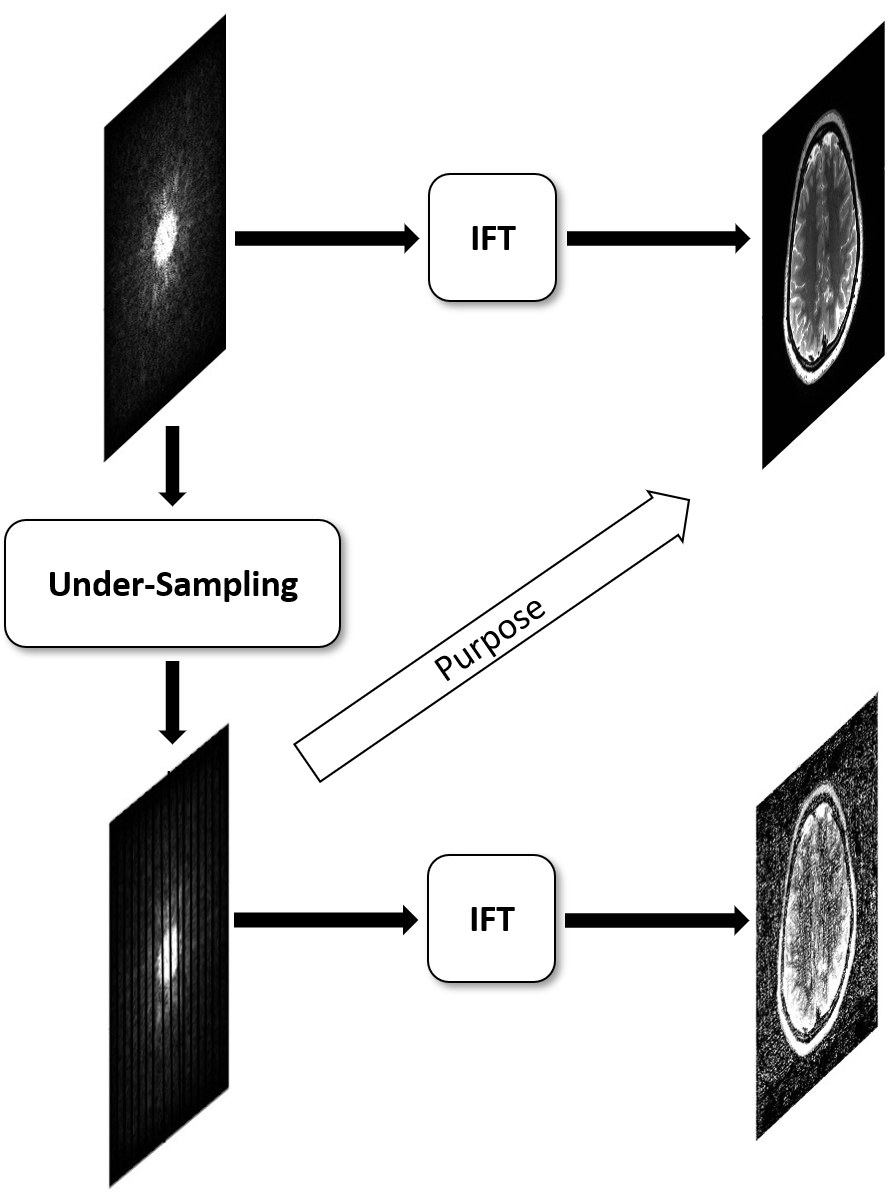
\includegraphics[width=0.3\linewidth]{chapters/chapter-3/figs/purpose-diagram}
	\caption{}
	\label{fig:purpose-diagram}
\end{figure}



















%\include{chapters/definitions}
%\include{chapters/literature}
%\chapter{نتایج}
%\include{chapters/conclusions}
\chapter{پیش زمینه تحقیق}\label{ch:background}

\section{ساختار تصویربرداری \mri}\label{sec:mri-basics}

\subsection{تاریخچه}


تاریخچه تصویربرداری تشدید مفناطیسی
\LTRfootnote{Magnetic Resonance Imaging}(\mri)
تلاش تعداد زیادی از محققانی را شامل می‌شود که پدیده تشدید مغناطیسی هسته
\LTRfootnote{Nuclear Magnetic Resonance}(\lr{NMR})
را کشف کردند.
در سال ۱۹۵۰، حصول تصویر یک بعدی \mri توسط هرمن کار 
\LTRfootnote{Herman Carr}
 گزارش گردید. پاول لاتربر 
\LTRfootnote{Paul C. Lauterbur}
، شیمیدان آمریکایی با کار بر روی تحقیقات پیشین، موفق به ابداع روش‌هایی برای تولید تصاویر دو بعدی و سه بعدی \mri گردید. سرانجام وی در سال ۱۹۷۳ اولین تصویر گرفته شده بر اساس تشدید مغناطیس هسته‌ای (\lr{NMR}) خود را منتشر نمود. اولین تصویر مقطع نگاری از یک موش زنده در ژانویه ۱۹۷۴ منتشر گردید.


از سوی دیگر تحقیقات و پیشرفت‌های مهمی در زمینهٔ تصویر برداری بر اساس تشدید مغناطیسی هسته برای نخستین بار در دانشگاه ناتینگهام انگلستان 
\LTRfootnote{University of Nottingham}
صورت پذیرفت، جایی که پیتر منسفیلد فیزیکدان برجستهٔ آن مؤسسه با گسترش یک روش ریاضی موفق به کاهش زمان تصویربرداری و افزایش کیفت تصاویر نسبت به روش بکارگرفته شده توسط لاتربر گردید. در همان زمان در سال ۱۹۷۱ دانشمند آمریکایی ارمنی تبار ریموند دامادیان استاد دانشگاه ایالتی نیویورک در مقاله‌ای که در مجلهٔ Science منتشر گردید، اعلام نمود که امکان تشخیص تومور از بافت‌های عادی به کمک تصویر برداری 
\lr{NMR}
 میسر می‌باشد.

سرانجام جایزهٔ نوبل پزشکی سال ۲۰۰۳ به خاطر اختراع ام آر آی به پاول لاتربر از دانشگاه ایلینوی در اوربانا شامپاین و پیتر منزفیلد از انگلستان اعطا گردید. 
این جایزه به تنهایی می‌تواند اهمیت این نوع تصویربرداری را نشان دهد.

اما چه عواملی باعث شده‌اند تا این‌قدر \mri بااهمیت و ویژه باشند؟ تصویربرداری \mri روشی غیر تهاجمی و نسبتا امن است. 

سیستم‌های ام آر آی امروزه غالباً دارای قدرت میدان‌های $0.2$، $1$ ، $1.5$ ، و $3$ تسلا می‌باشند.
در ایالات متحده آمریکا بیمارستان‌ها و مراکز خدمات بهداشتی اجازه استفاده از سیستم‌های تا $4$ تسلا را نیز برای یک بیمار دارند. اما از چهار تسلا به بالا صرفاً جنبه و کاربردهای تحقیقاتی دارد.

امروزه بزرگ‌ترین تولیدکننده‌های سیستم‌های ام آر آی شرکت‌های زیمنس (آلمان)، جنرال الکتریک (آمریکا)، توشیبا (ژاپن)، و فیلیپس (هلند) می‌باشند.

\subsection{خطرات \mri}
برخلاف سایر دستگاه‌های تصویربرداری مثل اشعه ایکس و سی‌تی اسکن، ام آر آی از تشعشع یونیزه استفاده نمی‌کند. از این ابزار می‌توان برای تصویربرداری از جنین در دوران بارداری استفاده کرد بدون آن که اثری روی آن داشته باشد. اما باز هم این روش ممکن است خطراتی در پی داشته باشد و به همین دلیل جوامع پزشکی استفاده از \mri را در مراحل اولیه تشخیص بیماری توصیه نمی‌کنند. از آن‌جایی که در فرآیند ام آر آی از مغناطیس قوی استفاده می‌شود هر قطعه فلزی که در بدن وجود داشته باشد مثل ضربان ساز قلب، مفصل مصنوعی، دریچه مصنوعی قلب، حلزون مصنوعی گوش و یا هر نوع صفحه و پیچ و مهره فلزی در بدن ممکن است خطرساز باشد، چون میدان مغناطیسی می‌تواند باعث جابجایی و یا گرم شدن آن قطعه شود.

تعدادی از بیمارانی که از ضربان ساز قلب استفاده می‌کردند طی انجام ام آر آی از دنیا رفتند. بنابراین لازم است تکنولوژیست \mri سوالات لازم را قبل از انجام این فرآیند از بیمار بپرسد. البته بیشتر قطعات فلزی که امروز در ایمپلنت‌های بدن استفاده می‌شوند تحت تأثیر میدان‌های مغناطیسی قرار نمی‌گیرند و به اصطلاح
\lr{MR-Safe}
 هستند. علاوه بر این، هنگام اسکن، دستگاه ام آر آی صداهای بلندی تولید می‌کند که ممکن است باعث ناراحتی فرد شود، بنابراین استفاده از حفاظ گوش در طول این فرآیند ضروری است.



\begin{figure}[t!]
	\centering
%	\copyrightbox[b]{
%	\begin{minipage}[c]{0.9\textwidth}
%	\centering
	\subfigure[تصویر پاول لاتربور]{
		\copyrightbox[b]{
		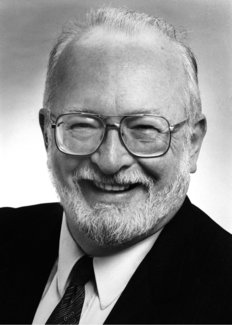
\includegraphics[height=0.36\linewidth]{chapters/chapter-2/figs/lauterbur-13686-content-portrait-mobile-tiny}
		}{\urlSource{https://is.gd/HgbMvo}}
		\label{subfig:paullauterbur}
	}
	\hspace{0.1\linewidth}
	\subfigure[تصویر هرمن کار]{
		\copyrightbox[b]{
		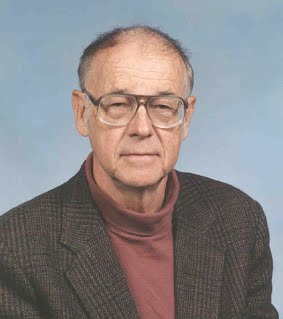
\includegraphics[height=0.36\linewidth]{chapters/chapter-2/figs/herman_carr}
		}{\urlSource{https://is.gd/teAHxS}}
		\label{subfig:herman-carr}
	}
	\hspace{0.1\linewidth}
	\subfigure[تصویر Peter-Mansfield]{
		\copyrightbox[b]{
			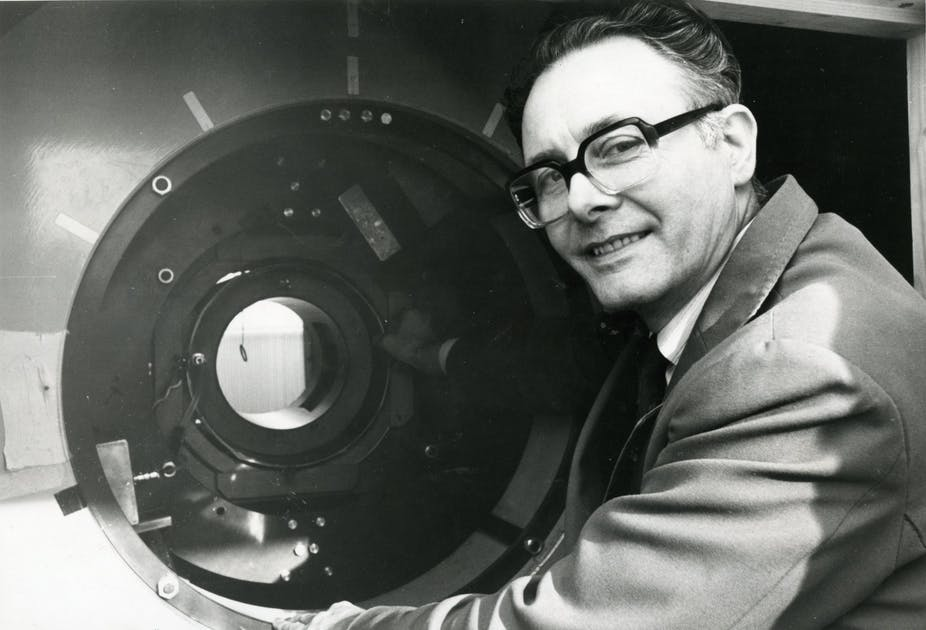
\includegraphics[height=0.36\linewidth]{chapters/chapter-2/figs/Peter-Mansfield}
		}{\urlSource{https://is.gd/W7AXIL}}
		\label{subfig:Peter-Mansfield}
	}


%	\end{minipage}
%	}{\scriptsize\url{https://www.nobelprize.org/prizes/medicine/2003/lauterbur/biographical/}
%		\url{https://sites.google.com/a/pbsd.k12.pa.us/magnetic-resonance-imaging/herman-carr}
%		\url{https://theconversation.com/obituary-professor-sir-peter-mansfield-whose-invention-of-the-mri-scanner-revolutionised-medicine-72815}}
	\caption{تصویر سازندگان اصلی دستگاه تصویربرداری \mri}
	
	
\end{figure}



\begin{figure}
	\centering
	\copyrightbox[b]{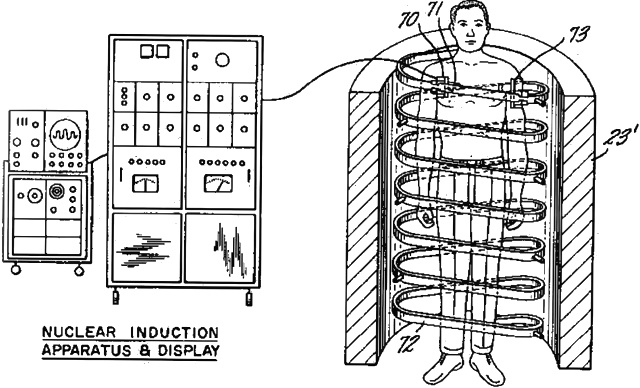
\includegraphics[width=0.6\linewidth]{chapters/chapter-2/figs/Damadian_invention}}
	{\urlSource{https://w.wiki/3STS}}
	\caption{تصویری از آرشیو اداره ثبت اختراعات آمریکا که متعلق به ریموند دامادیان، دانشمند آمریکایی و یکی از مخترعین سیستم‌های نوین ام آر آی}
	\label{fig:Damadian_invention}
\end{figure}


\subsection{تولید کنندگان بزرگ دستگاه \mri}

دستگاه های \mri توسط کمپانی های مختلفی در دنیا تولید ‌میشوند. هر یکی از این دستگاه ها ملاحظاتی دارند که با دیگری متفاوت است. در این قسمت صرفا برای شناخت، تعدادی از فروشندگان دستگاه \mri
\LTRfootnote{MR vendors}
 نام برده می‌شود و وارد جزئیات این تفاوت ها نمی‌شویم.  
 شکل \ref{fig:siemens-espree-mri}
یک دستگاه \mri ساخته شده توسط \lr{SIEMENS}
را نشان می‌دهد.

\begin{figure}[t!]
	\centering
	\copyrightbox[b]{
		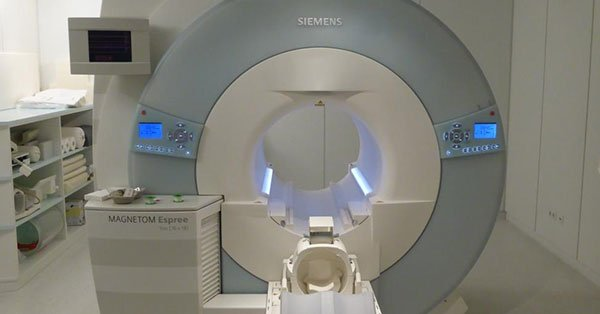
\includegraphics[width=0.7\linewidth]{chapters/chapter-2/figs/siemens-espree-mri}
	}{\urlSource{https://is.gd/q4EXoV}} 
	\removevspace[1]
	\caption{یک دستگاه \mri ساخت شرکت \lr{SIEMENS}}
	\label{fig:siemens-espree-mri}
\end{figure}


برخی از مهمترین شرکت های تولید کننده دستگاه \mri در زیر لیست شده اند.

\begin{multicols}{2}
	\footnotesize
	\begin{itemize}
		\item \lr{GE Healthcare}
		\item \lr{Philips}
		\item \lr{Siemens Healthcare}
		\item \lr{Toshiba Medical Systems Corporation}
		\item \lr{Fujifilm Holdings}
		\item \lr{Shimadzu Corporation}
		\item \lr{Carestream Health}
		\item \lr{Hitachi Medical Corporation}
		\item \lr{Hologic}
		\item \lr{Esaote}
	\end{itemize}
\end{multicols}


\subsection{زبان فنی \mri}
در حوزه \mri نیز مانند دیگر شاخه های علوم پزشکی و کلا علوم، زبان و عبارت های خاص خود را دارد. بسیاری از این عبارت ها که با حرف \lr{T} شروع می‌شوند ممکن است کمی عجیب و سردم کننده باشد. هرچند در ادامه برخی از آن‌ها را به تفصیل توضیح خواهیم داد اما در ابتدا یک بار با آن ها در این قسمت آشنا می‌شویم. جدول \ref{table:overview-mri-terms}
برگرفته شده از \cite{book:MRIfromPictureToProton}
این موارد را بیان می‌کند.

\begin{table}[b!]
	\centering
	\rowcolors{2}{gray!10}{white}
	\begin{tabularx}{\textwidth}{|c|X|}
		\hline\rowcolor{headerColor}
		عبارت & توضیحات \\\hline
		\lr{\Tone} & 
		یکی از مشخصه های یک بافت است که \textit{زمان آزادسازی اسپین-لتیس} نامیده می‌شود.
		\\
		\lr{\Ttwo} & 
		یکی از مشخصه های یک بافت است که \textit{زمان آزادسازی اسپین-اسپین} نامیده می‌شود.
		\\
		\lr{\TtwoStar} & 
		یکی از مشخصه های بافتی است که در یک میدان مغناطیسی قرار دارد و \textit{زمان آزادسازی اسپین-اسپین آشکار} نامیده می‌شود.	
		\\
		\lr{PD} & 
		یکی از مشخصه های بافت است که چگالی پروتون نامیده می‌شود(ارتباط نزدیکی با محتوای آبی دارد).
		\\
		\lr{TR} & 
		یکی از مشخصه های زمانی اسکن است که زمان تکرار نامیده می‌شود.
		\\
		\lr{TE} & 
		یکی از مشخصه های زمانی اسکن است که زمان وارونگی نامیده می‌شود.
		\\
		\lr{TI} & 
		یکی از مشخصه های زمانی اسکن است که زمان تکرار نامیده می‌شود.
		\\
		$\alpha$ & 
		یکی از پارامتر های اسکن است که زاویه تکان نیز نامیده می‌شود.
		\\
		\lr{{\Tone}w} & 
		توصیفی از کانتراست تصویر است که بستگی شدیدی به خاصیت \Tone بافت دارد.
		\\
		\lr{{\Ttwo}w} & 
			توصیفی از کانتراست تصویر است که بستگی شدیدی به خاصیت \Ttwo بافت دارد.
		\\
		\lr{{\TtwoStar}w} & 
			توصیفی از کانتراست تصویر است که بستگی شدیدی به خاصیت \TtwoStar بافت دارد.
		\\
		\lr{PDw} & 
			توصیفی از کانتراست تصویر است که بستگی شدیدی به خاصیت \lr{PD} بافت دارد.
		\\\hline
	\end{tabularx}
	\caption{عبارت مهم در \mri}
	\label{table:overview-mri-terms}
\end{table}

\subsection{بررسی مفهوم اسپین}
 

ساختار یک اتم، یکی از اجزای اساسی در آزمایشات تشدید مغناطیسی است. اتم ها از سه ذره اصلی 
\LTRfootnote{Fundamental Particles}
تشکیلی شده اند:
\begin{enuminline}
	\item پروتون، که بار مثبت دارد
	\item نوترون، که بدون بار است
	\item الکترون، که بار الکتریکی منفی دارد
\end{enuminline}.
پروتون‌ها و نوترون‌ها در درون هسته اتم قرار گرفته اند و الکترون‌ها در خارج هسته به دور آن می‌گردند.
همچنین \textit{عدد‌اتمی}
\LTRfootnote{Atomic Number}
تعداد پروتون‌های یک اتم و \textit{جرم‌اتمی}
\LTRfootnote{Atomic Weight}
، تعداد پروتون‌ها و نوترون‌ها در یک اتم را نشان می‌دهد. اگر دو اتم عدد‌‌اتمی یکسان اما عدد جرمی متفاوت داشته باشند، آن دو اتم را \textit{همریخت} یا \textit{ایزوتوپ}
\LTRfootnote{Isotope}
یکدیگر می‌نامند. که خواص شیمیایی مشابهی اما با نرخ‌های متفاوت دارند.


\begin{figure}[t]
	\centering
	\subfigure[اسپین]{		
		\copyrightbox[b]{
			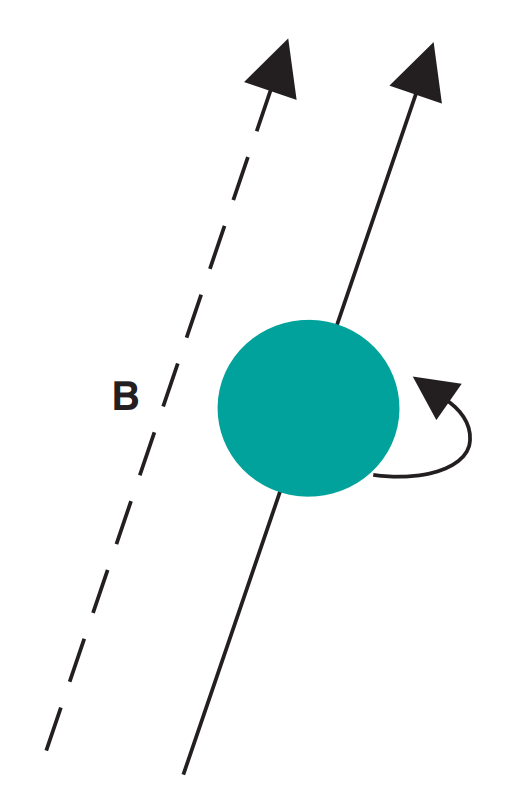
\includegraphics[height=0.3\linewidth]{chapters/chapter-2/figs/one-spin}
		}{\scriptsize\Doi{10.1002/9781119013068}}
		\label{fig:one-spin}}
		\hspace{0.2\linewidth}
	\subfigure[مغناطیس]{
		\copyrightbox[b]{
			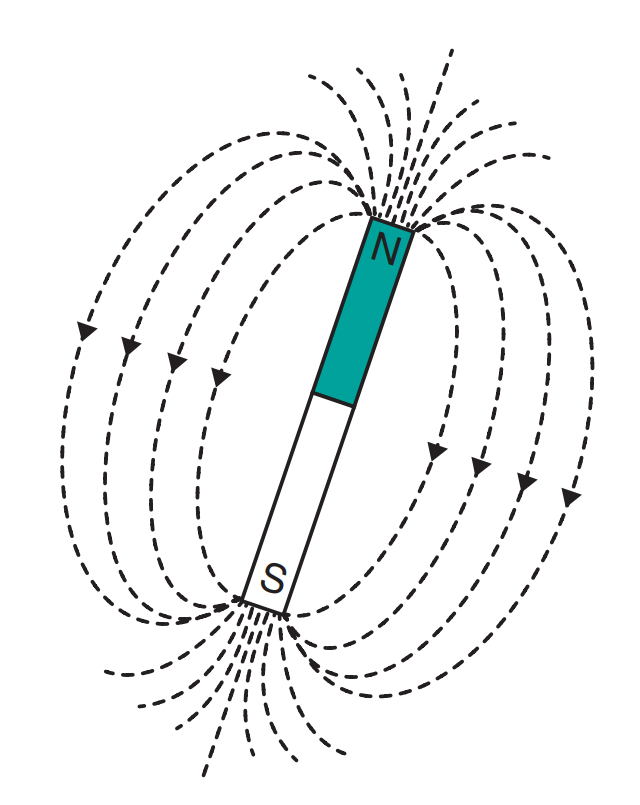
\includegraphics[height=0.3\linewidth]{chapters/chapter-2/figs/one-magnet}
		}{\scriptsize\Doi{10.1002/9781119013068}}
		\label{fig:one-magnet}}
	\caption{} 
\end{figure}

یکی دیگر از خواص هسته‌ها، اسپین
\index{اسپین}
\LTRfootnote{Spin}
یا اندازه حرکت زاویه ای ذاتی اسپینی
\LTRfootnote{Intrinsic Spin Angular Momentum}
است.
هسته هایی که حرکت اسپینی دارند همواره حول یک محور درحال گردش هستند.(شکل \ref{fig:one-spin} حرکت اسپینی را نمایش می‌دهد.)
تمام عناصر جدول تناوبی
\LTRfootnote{Periodic Table}
بجز آرگون
\LTRfootnote{Argon}
و سریم
\LTRfootnote{Cerium}
حداقل یک ایزوتوپ دارند که حرکت اسپینی دارد. از آنجا که این حرکت نقش مهمی در اصول تصویربرداری \mri دارد، بنابراین تقریبا تمامی عناصر قابلیت مشاهده شدن در تصویربرداری \mri را دارند. اسپین یکی از خواص کوانتومی هسته است و تعداد محدودی اسپین در طبیعت وجود دارند. 

\begin{table}[b]
	\centering
	\begin{tabular}{|C{5em}|C{5em}||C{14em}|}
		\hline \rowcolor{headerColor}
		
		عدد اتمی & جرم اتمی & عدد اسپین
		\\\hline\hline
		زوج & زوج & صفر \\\hline
		فرد & زوج & عدد صحیح \\\hline
		فرد & 
		\multirow{2}{*}{فرد}
		 & 
		\multirow{2}{*}{عدد صحیح و نصفی}
		\\\cline{0-0}
		زوج &  &
		\\\hline
	\end{tabular}
	\caption{بررسی عدد اسپین نسبت به عدد اتمی و جرم اتمی }
	\label{table:spin-even-odd}
\end{table}

\begin{table}[b]
	\centering
	\begin{tabular}{|C{5em}|C{5em}||C{14em}|}
		\hline \rowcolor{headerColor}
		
		تعداد پروتون & تعداد نوترون & عدد اسپین
		\\\hline\hline
		زوج & زوج & صفر \\\hline
		فرد & فرد & عدد صحیح \\\hline
		فرد & زوج & 
		\multirow{2}{*}{عدد صحیح و نصفی}
		\\\cline{0-1}
		زوج & فرد &
		\\\hline
	\end{tabular}
	\caption{بررسی عدد اسپین نسبت به تعداد پروتون‌ها و تعداد نوترون ها }
	\label{table:spin-even-odd-pn}
\end{table}

اسپین که با نماد $I$ و یا $\Phi$ نمایش می‌دهند، مقدایر کوانتیده‌ای به خود می‌گیرد به طوری که می‌تواند صفر یا یک عدد صحیح (مثل $1$و $2$و $3$و ...) و یا یک عدد صحیح و نصفی (مثل $0.5$و $1.5$و $2.5$ و ...) باشد. 
بنابر \cite{book:basic-principles-and-applications}، می‌توان جدول 
\ref{table:spin-even-odd}
را استخراج نمود که آن را می‌توان به شیوه جدول \ref{table:spin-even-odd-pn}
برحسب تعداد پروتون ها و نوترون ها به خاطر سپرد.
درحقیقت اتم‌هایی با عدد اتمی یا جرم اتمی فرد دارای اسپین هستند و اگر هردو زوج باشند، نمی‌توان آن‌ها را در تصویربرداری \mri مطالعه نمود. 

در تصویر برداری \mri ما برروی هسته‌هایی متمرکز هستیم که اسپین آن‌ها \f12 است. به‌طور خاص  در تصویربرداری \mri، هسته اتم هیدروژن
\ce{^1_1H}
(فراوان‌ترین ایزوتوپ هیدروژن) و اتم کربن
\ce{^{13}_6C}
(ایزوتوپ کمیاب اما مفید در تصویربرداری) استفاده می‌شود.\cite{Handouts-NMRhandout.html}
با توجه به این که فراوان ترین ایزوتوپ کربن یعنی 
\ce{^{12}_6C}
فاقد اسپین است (چراکه تعداد پروتون ها و نوتورون های آن هردو زوج هستند)، بنابراین قابل بررسی در تصویربرداری  \mri نیستند. البته عناصر دیگری نیز مانند 
\ce{^19_9F}،
\ce{^23_11Na} و
\ce{^31_15P}
نیز در این تصویربرداری حائز اهمیت می‌باشند.

% READ THIS: http://iverson.cm.utexas.edu/courses/310N/Handouts/NMRhandout.html

اتم هیدروژن 
\ce{^1_1H}
از آن جهت بسیار اهمیت دارد که اولا ساختار بسیار ساده‌ای دارد (هسته آن از یک تک پروتون تشکیل شده است) و ثانیا در ساختمان اصلی آب 
\ce{H2O}
بکار رفته‌است.
بدن هر‌انسان به طور میانگین، از 60 درصد آب تشکیل شده است. همچنین برخی ارگان های بدن حتی تا 90 درصد از آب ساخته شده‌اند. مغز و قلب انسان 73 درصد آب، ریه ها 83 درصد، پوست 64 درصد، ماهیچه‌ها و کلیه‌ها 79 درصد و استخوان ها 31 درصد آب را شامل می‌شوند.\cite{science-water-you-water-and-human-body}
از این رو، اتم هیدروژن نقش تعیین کننده ای دارد. از آن‌جایی که اتم اکسیژن \ce{^16_8O} اسپینی ندارد، بنابراین نقشی در تصویربرداری \mri ندارد. با توجه یه این که آب در بافت های نرم به میزان بیشتری وجود دارد، این نوع تصویر برداری عموما برای تصویربرداری از نواحی دارای بافت نرم مانند مغز مورد استفاده قرار می‌گیرد.

از آنجایی که درون هسته متشکل از پروتون هاست، بارالکتریکی هسته مثبت است. از این رو، در صورت حرکت دورانی حول محور دوران خود، یک میدان مغناطیسی هم‌راستا با همان محور دوران، ایجاد می‌کند. جون‌که مقدار اندازه اسپین هسته یک مقدار ثابت است این میدان مغناطیسی نیز اندازه ثابتی دارد. بنابراین برای ممان مغناطیسی هسته
\LTRfootnote{Nuclear Magnetic Moment} 
دو مولفه‌ی مقدار و جهت میدان مغناطیسی می‌توان تعریف کرد. به عبارت دیگر یک هسته دارای اسپین را می‌توان به صورت یک آهن‌ربای میکروسکوپیک ریز درنظر گرفت
(شکل \ref{fig:one-magnet}).
به این آهنرباهای کوچک ایزوکرومات (اسپینی)
\LTRfootnote{(spin) isochromats}
 گفته می‌شود. \cite{SpinEchoMagnetic2013}
برای یک پروتون یا همان هسته ی \ce{^1_1H}، ممان مغناطیسی $\mu$ و تکانه زاویه‌ای اسپینی
\LTRfootnote{Spin Angular Momentum}$\Phi$
با یک ثابت تناسب $\gamma$ به صورت زیر به یک دیگر مرتبط می‌شوند.

\removevspace
\begin{equation}\label{eq:mu=gamma.phi}
	\mu = \gamma . \Phi
\end{equation}

که $\gamma$ در رابطه‌ی بالا نسبت ژایرومغناطیسی 
\LTRfootnote{Gyromagnetic Ratio}
نامیده می‌شود و واحد  $\frac{\gamma}{2\pi}$
را عموما برحسب (\lr{MHz/Tesla})

بیان می‌کنند.



\begin{figure}[t]
	\centering
	\copyrightbox[b]{
		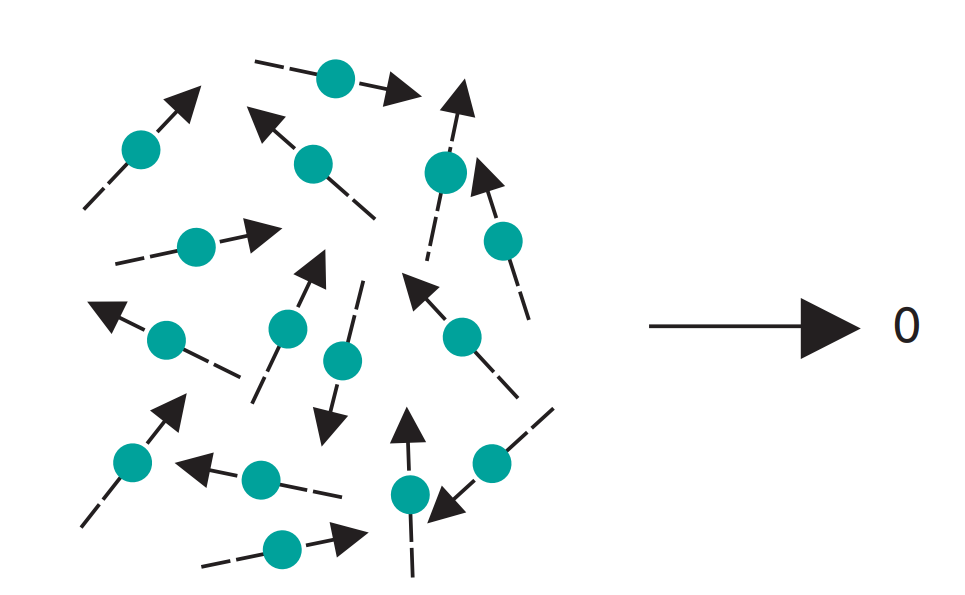
\includegraphics[width=0.5\linewidth]{chapters/chapter-2/figs/balance-spin}
	}{\scriptsize\Doi{10.1002/9781119013068}}
	\caption{}
	\label{fig:balance-spin}
\end{figure}


در اندازه گیری \mr مجموعه‌ای از این میدان های مغناطیسی کوچک مورد بررسی قرار می‌گیرد و به صورت تکی به قدری نیستند که بتوان آن‌ها را بررسی نمود. جهت این اسپین ها یک مکانیسم تصادفی دارد به طوری که در یک مجموعه هسته دارای اسپین، در صورت عدم حضور میدان خارجی، برایند میدان مغناطیسی حاصل در آن مجمموعه صفر است و سیستم درحالت تعادل قرار دارد. 
(شکل \ref{fig:balance-spin}) در واقع تصاویر \mri در ابعاد ماکروسکوپیک ثبت می‌شوند.


\begin{figure}
	\centering
	\copyrightbox[b]{
		\centering
		\begin{minipage}{0.9\linewidth}
				\centering
				\subfigure[]{
				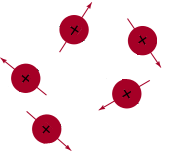
\includegraphics[height=0.25\linewidth]{chapters/chapter-2/figs/alineamiento-no}	
				\label{subfig:alineamiento-no}}		
				\hspace{0.15\linewidth}
				\subfigure[]{
				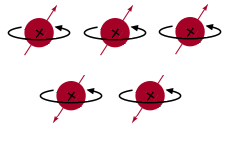
\includegraphics[height=0.22\linewidth]{chapters/chapter-2/figs/alineamiento-yes}	
				\label{subfig:alineamiento-yes}} 
		\end{minipage}	
	}{\urlSource{https://is.gd/XTUru4}}%http://www.qorganica.es/QOT/T12/alineamiento_e_exported/index.html
	\caption{}
	\label{fig:alineamiento}
\end{figure}



\begin{figure}
	\centering	
	\subfigure[]{
	\copyrightbox[b]{
		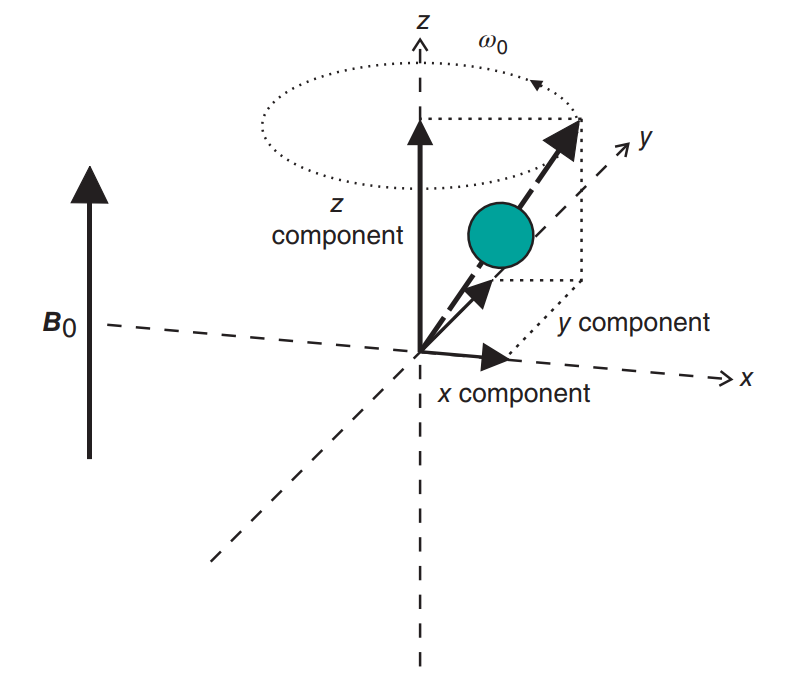
\includegraphics[height=0.35\linewidth]{chapters/chapter-2/figs/B-spin}	
		\label{subfig:precession-spin}
	}{\scriptsize\Doi{10.1002/9781119013068}}}
	\hspace{0.1\linewidth}
	\subfigure[]{
	\copyrightbox[b]{
		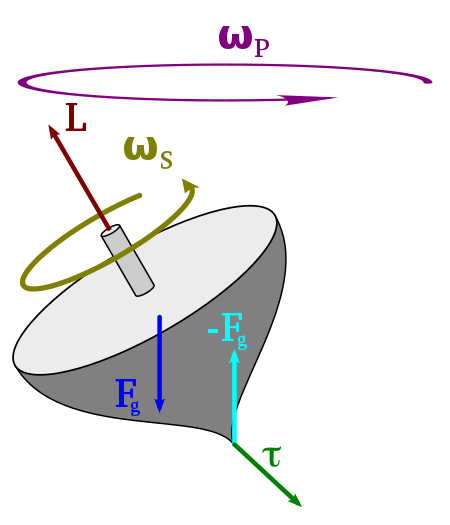
\includegraphics[height=0.28\linewidth]{chapters/chapter-2/figs/PrecessionOfATop}	
		\label{subfig:precession-top}
	}{\urlSource{https://w.wiki/3TPJ}}}
	\caption{}
	\label{fig:precession}

\end{figure}

\subsubsection{پروتون‌ها در یک میدان مغناطیسی خارجی}


هنگامی که پروتون‌های دارای اسپین در داخل یک \textit{میدان مغناطیسی قوی }
\RTLfootnote{
هنگامی که از میدان مغناطیسی قوی صحبت می‌کنیم منظور چیزی حدود حداقل $1$ تسلا یا $10000$ گاوس است. 
}
خارجی $B_0$ قرار می‌گیرند، دو اتفاق مهم رخ می‌دهد: اولا ممان های مغناطیسی اتم ها تمایل پیدا می‌کنند که\textit{هم‌جهت} یا \textit{خلاف جهت} 
\LTRfootnote{Parallel or Anti-parallel}
قرار بگیرند (شکل \ref{subfig:alineamiento-yes})
و ثانیا وادار می‌شوند که حرکت چرخشی حول راستای میدان مغناطیسی خارجی داشته باشند که به این پدیده \textbf{حرکت تقدیمی}
\LTRfootnote{Precession}
می‌گویند. 

\begin{figure}
	\centering\copyrightbox[b]{
		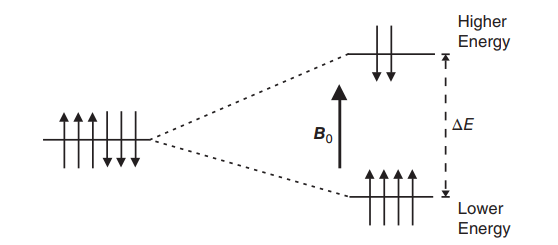
\includegraphics[width=0.6\linewidth]{chapters/chapter-2/figs/zeeman-diagram}
	}{\scriptsize\Doi{10.1002/9781119013068}}
	\caption{}
	\label{fig:zeeman-diagram}
\end{figure}


همانطور که اشاره شد در اثر یک میدان مغناطیسی خارجی $B_0$ تمایل پیدا می‌کنند که ممان‌های مغناطیسی خود را در جهت یا خلاف جهت آن میدان قرار دهند. آن‌هایی که در جهت آن میدان قرار داشته باشند انرژی کمتر و آن‌هایی که در خلاف جهت آن میدان باشند، انرژی بیشتری را دارا می‌باشند.  تعداد پروتون های زیادی وجود دارند که در جهت و یا خلاف جهت میدان قرار می‌گیرند و تعداد آن ها تقریبا مشابه هم دیگر است که در حقیقت می‌توان گفت اکثر پروتون ها در اثر این میدان  اثر یک دیگر را خنثی می‌کنند اما برایند آن ها صفر نمی‌شود زیرا تعداد آنانی که در جهت میدان قرار می‌گیرند به میزان کمی، بیشتر است که به آن به اصطلاح، \textbf{اسپین اضافه}
\LTRfootnote{Excess Spin}
گفته می‌شود.
(شکل \ref{fig:zeeman-diagram})
از این رو مقدار ناصفری برای \textbf{مغناطیس‌شوندگی شبکه} 
\LTRfootnote{Net Magnitation}
وجود دارد.
به عبارت دقیق‌تر، نسبت 
\RLE{$\frac{\rltext{تعداد هم‌جهت‌ها} - \rltext{تعداد خلاف جهت‌‌ها}}{\rltext{تعداد کل پروتون‌ها}}$}
یک عدد نامنفی بسیار کوچک است. به عنوان مثال، در یک میدان مغناطیسی خارجی $B_0 = 3 \mathrm{T}$ و در دمای اتاق، نسبت مذکور چیزی در حدود $10^{-5}$ می‌باشد. یعنی از یک میلیون پروتونی که در اختیار داریم تنها 10 تای آنان در اسپین اضافه نقش دارند که آن اسپین اضافه در تولید \textbf{سیگنال های \mr}\LTRfootnote{MR Signals}
استفاده می‌شوند.
\begin{figure}
	\centering
	\copyrightbox[b]{
		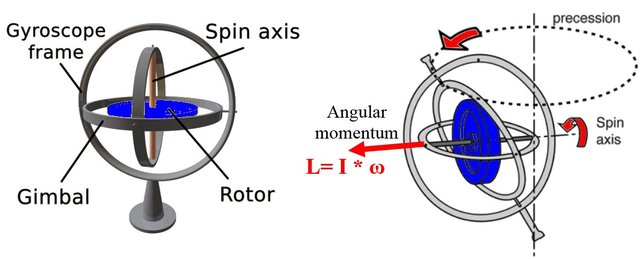
\includegraphics[width=0.7\linewidth]{chapters/chapter-2/figs/Gyroscope-components}
	}{\urlSource{https://is.gd/T3UkHu}}
	\caption{}
	\label{fig:gyroscope-components}
\end{figure}

به طور دقیق تر تعداد پروتون‌های همجهت ($N_\text{down}$) و خلاف جهت میدان ($N_\text{up}$)، از رابطه‌‌ی زیر محاسبه می‌گردد.
 
 \removevspace
 \begin{equation}
 	\dfrac{N_\text{up}}{N_\text{down}} = e^{\frac{\Delta E}{k_B T}}
 \end{equation}

که در این رابطه، $k_B$ ثابت بولتزمن
\LTRfootnote{Boltzmann Constant}
($k_B = 1.38 × 10^{–23} \mathrm{J} \mathrm{K}^{-1}$)
 و $\Delta E$ اختلاف این دو سطح انرژی است که در شکل \ref{fig:zeeman-diagram}
 مشخص شده است و $T$ نیز دما بر حسب کلوین می‌باشد. مرجع \cite{McRobbie}
 روابط کوانتومی دقیق تری را در این رابطه بیان کرده است.
 
 
پدیده دومی که در اثر قرار گرفتن یک پروتون در درون یک میدان مغناطیسی بسیار قوی برایش اتفاق می‌افتد، \textbf{حرکت تقدیمی }نامیده می‌شود. این پدیده را می‌توان به صورت یک ژایروسکوپ 
(\ref{fig:gyroscope-components})
(شکل \ref{subfig:precession-top}) و یا حرکت آشنای یک فرفره‌ی درحال گردش (شکل \ref{subfig:precession-top})
در نظر گرفت. اگر یک ژیروسکوپ و یا فرفره در راستای عمودی جهت گیری داشته باشد، بدون تلوتلو‌خوردن
\LTRfootnote{Wobbling}
به دور خود می‌چرخد. هنگامی که یک بار محور چرخش ژیروسکوپ از محور عمومی فاصله بگیرد، در اثر میدان مغناطیسی زمین یا همان جاذبه
\LTRfootnote{Gravity}
 شروع به گردش حول محور عمودی خود با فرکانسی مستقل از فرکانس اسپینی مطابق شکل \ref{subfig:precession-top}
می‌کند. 

به‌طور‌خلاصه دو نوع حرکت برای یک پروتون دارای اسپین در یک میدان مغناطیسی قوی می‌توان تصور کرد.

\begin{alphabetlist}
	\item
	حرکت \textbf{اسپینی} هسته به دور محور خود و با فرکانس مخصوص خود که آن حرکت، \textbf{ممان زاویه‌ای اسپینی }را تولید می‌کند و آن نیز باعث ایجاد \textbf{ممان مغناطیسی }می‌شود.
	\item
	حرکت \textbf{تقدیمی} که نوعی تلوتلو خوردن و  گردش حول یک محور دیگز و با فرکانسی مستقل می‌باشد.
\end{alphabetlist}


\subsubsection{مغناطش شبکه}


\begin{figure}
	\centering
	\copyrightbox[b]{
		\begin{minipage}{0.8\linewidth}\centering
			\subfigure[]{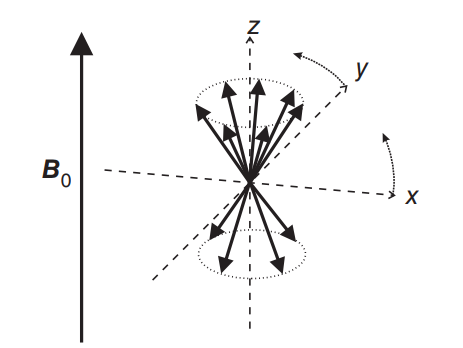
\includegraphics[height=0.3\linewidth]{chapters/chapter-2/figs/net-mag-a}\label{subfig:net-mag-a}}
			\hspace{0.15\linewidth}
			\subfigure[]{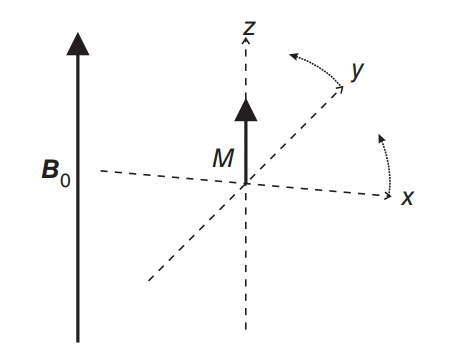
\includegraphics[height=0.3\linewidth]{chapters/chapter-2/figs/net-mag-b}\label{subfig:net-mag-b}}
		\end{minipage}
	}{\scriptsize\Doi{10.1002/9781119013068}}
	\caption{}
	\label{fig:net-mag}
\end{figure}


\textbf{مغناطش شبکه} و یا \textbf{مغناطیس‌شوندگی شبکه} 
\LTRfootnote{Net Magnetization}
موضوع مهم دیگری است که در \mri مطرح می‌شود.
مغناطیس شوندگی هر پروتون را می‌توان به عنوان یک بردار در‌نظر گرفت. \textbf{مغناطش شبکه} را می‌توان به‌عنوان برایند آن بردار ها مطابق شکل \ref{fig:net-mag}در نظر گرفت. 
هر یک از این بردار را می‌توان در راستای میدان به دو مولفه‌ی طولی و عرضی تجزیه نمود. با این مدل‌سازی نیز همان‌طور که پیشتر نیز توضیح داده شد، اکثر مولفه هایی هم‌جهت و خلاف جهت، هم‌دیگر را کنسل می‌کنند و تعداد کمی اسپین های هم‌جهت باقی می‌مانند که اسپین اضافه نام داشتند. اما موله‌عرضی صفر است. چراکه اسپین پروتون‌ها فاز تصادفی دارند و بنابراین برایند آنان صفر می‌شود. این یعنی مغناطش شبکه، مولفه‌ای در راستای عرضی ندارد و صرفا در راستای مولفه‌ی طولی یا همان راستای میدان مغناطیسی خارجی $B_0$ می‌باشد. (شکل \ref{subfig:net-mag-b})

\subsubsection{ فرکانس لامور و پدیده \nmr}

همانند رابطه‌ی بین تکانه زاویه ای اسپینی و ممان مغناطیسی که در رابطه‌ی \ref{eq:mu=gamma.phi} بیان شد، رابطه تناسبی دیگری نیز بین فرکانس زاویه‌ای حرکت تقدیمی $\omega_0$ و میدان مغناطیسی خارجی $B_0$  
با \textbf{ثابت تناسب ژایرومغناطیسی}
\LTRfootnote{Constant Gyromagnetic Ratio}
$\gamma$
می‌توان استخراج نمود:


\removevspace
\begin{equation}\label{eq:larmor}
	\omega_0 = \gamma . B_0 \quad \leftrightarrow \quad f_0 = \frac{\gamma}{2\pi}. B_0
\end{equation}

به عنوان یک مثال، به ازای میدان خارجی $B_0=1 \mathrm{T}$، مقدار $f_0$ برابر $42.58 \mathrm{MHz}$ می‌شود. این فرکانس در شکل \ref{subfig:precession-spin}
نیز نشان داده شده است.
تساوی بالا به‌عنوان \textbf{تساوی لارمور}
\LTRfootnote{Larmor Equation}
شناخته می‌شود و مهم‌ترین معادله ای است که اکثر پدیده‌های مرتبط با \mri را توضیح می‌دهد که از بین آن پدیده‌ها میتوان به رزونانس مغناطیسی و قسمت های تصویر‌برداری مانند مفهوم میدان گرادیان و نقش آن در تصویر‌برداری اشاره نمود. ثابت تناسب ژایرومغناطیسی برخی از مهمترین عناصر در کاربرد \mri در جدول \ref{table:nmr-common} آورده شده است.


\begin{table}[!b]
	\centering
	\copyrightbox[b]{
	\begin{latin}
		\footnotesize
		\begin{tabularx}{\textwidth}{ | c | c | c | Y | Y | Y | Y | }
			\hline\rowcolor{headerColor}
			Element & Isotope & Spin & Natural Abundance & Quadrupole Moment, Q $(10^{-30} \frac{\mathrm{rad}}{m^2}\mathrm{A})$& Gyromagnetic Ratio $(10^7 \frac{\mathrm{rad}}{Ts})$ & Common Reference Standard\\ \hline\hline
			\multirow{2}{*}{Hydrogen} & \ce{^1_1H} & \f12 & 100 & 0 & 26.75105 & \ce{Si(CH3)4} \\ \cline{2-7}
			& \ce{^2_1H} or \ce{^2_1D}
			& 1 & < 0.1 & 2.8E-3 & 4.10646 & \ce{Si(CD3)4} \\ \hline
			\multirow{2}{*}{Boron} & \ce{^10_5B} & 3 & 19.7 & 0.08 & 2.87471 & \ce{BF3.OEt2} \\ \cline{2-7}
			& \ce{^11_5B} & \f32 & 80.3 & 0.04 & 8.58406 & \ce{BF3.OEt2} \\ \hline
			Carbon & \ce{^13_6C} & \f12 & 1.1 & 0 & 6.72804 & \ce{Si(CH3)4} \\ \hline
			\multirow{2}{*}{Nitrogen} & \ce{^14_7N} & 1 & 99.6 & 1 & 1.93297 & \ce{CH3NO2} \\ \cline{2-7}
			& \ce{^15_7N} & \f12 & 0.4 & 0 & -2.71171 & \ce{CH3NO2} \\ \hline
			Fluorine & \ce{^19_9F} & \f12 & 100 & 0 & 25.18034 & \ce{CFCl3} \\ \hline
			Aluminium & \ce{^27_13Al} & \f52 & 100 & 15 & 6.97594 & \ce{Al(NO3)3} in \ce{D2O} \\ \hline
			Silicon & \ce{^29_14Si} & \f12 & 4.7 & 0 & -5.3146 & \ce{Si(CH3)4} \\ \hline
			Phosphorus & \ce{^31_15P} & \f12 & 100 & 0 & 10.84015 & 85\% \ce{H3PO4} \\ \hline
			\multirow{2}{*}{Chlorine} & \ce{^35_17Cl} & \f32 & 75.5 & -7.9 & 2.62401 &\ce{NaCl} in \ce{D2O} \\ \cline{2-7}
			& \ce{^37_17Cl} & \f32 & 24.5 & -6.2 & 2.18428 & \ce{NaCl} in \ce{D2O} \\ \hline
		\end{tabularx}
	\end{latin}
	}{\urlSource{http://www.acadiau.ca/~bellis/resources/nmr/isotopes.html}}
	\vspace*{-2.5em}
	\caption{}\label{table:nmr-common}
\end{table}


\begin{figure}
	\centering
	\copyrightbox[b]{
		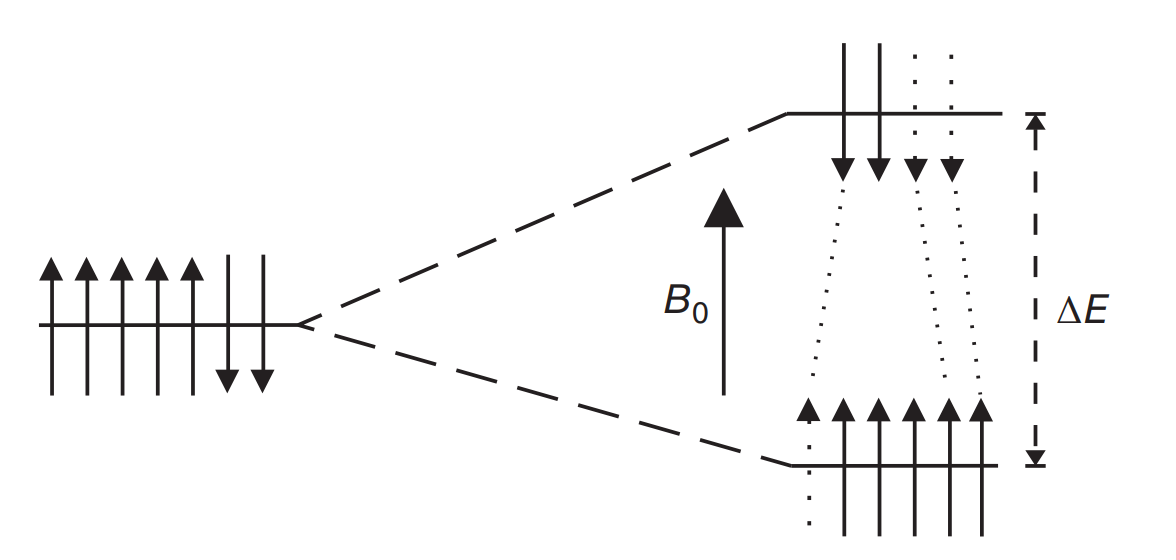
\includegraphics[width=0.6\linewidth]{chapters/chapter-2/figs/Energy-absorption}
	}{\scriptsize\Doi{10.1002/9781119013068}}
	\caption{}
	\label{fig:energy-absorption}
\end{figure}

گفته شد که براثر وارد کردن یک میدان خارجی $B_0$ بر مجموعه ای از پروتون ها تعدادی از آن اسپین ها همجهت با میدان می‌شوند که انرژی کمتری دارند و تعدادی از آنان نیز خلاف انرژی میدان جهت گیری می‌کنند که انرژی بیشتری را دارا می‌باشند و در هردو سطح انرژی
\LTRfootnote{Energy State}
دارای حرکت تقدیمی با فرکانس تقدیمی لارمور که از رابطه‌ی \ref{eq:larmor}
ناشی می‌شود، می‌باشند و اکثر آن ممان های مغناطیسی هم‌دیگر را خنثی می‌کردند و مغناطش شبکه که مقداری کوچک ولی ناصفری بود را بوجود می‌آوردند. 



در این هنگام اگر یک سیگنال الکترومغناطیسی \lr{RF}
\LTRfootnote{RadioFrequency}
با همان فرکانس لارمور $\omega_0$
به آن تابیده شود، مطابق شکل \ref{fig:energy-absorption}
تعدادی از اسپین هایی که هم جهت با میدان $B_0$ و در سطح انرژی پایین تری قرار داشتند، در اثر این تشدید، انرژی آن سیگنال را جذب می‌کنند و به سطح بالایی انرژی می‌روند که در این حالت نیز خلاف جهت میدان جهت گیری می‌کنند. این خاضیت در حقیقت یک ویژگی کوانتومی است که با فیزیک کلاسیک نمی‌توان آن را توجیه کرد و به عنوان وارونه‌سازی جمعیت
\LTRfootnote{Population Inversion}
شناخته می‌شود.



در اثر این اتفاق، مغناطش شبکه نیز دجار تغییر می‌شود. برای بررسی این تغییرات معمولا ساده تر است که دستگاه مختصات جدید $x'oy'$ 
را به شیوه زیر تعریف کنیم:

\removevspace
\begin{subequations}
\begin{align}\label{eq:x'oy'}
	x' &= x \cos(\omega_0 t) - y \sin(\omega_0 t) \\ 
	y' &= x \sin(\omega_0 t) + y \cos(\omega_0 t) \\ 
	z' &= z 
\end{align}
\end{subequations}

توجه داریم که در تعریف این دستگاه جدید پارامتر $t$ که همان زمان است، دخیل شده است و این یعنی
که دستگاه  مختصاتی در طول زمان با همان فرکانس لارمور $\omega_0$ در حال گردش است که شکل \ref{subfig:rotating-axis-x'oy'} آن را نشان می‌دهد.(محور $z$ ها در همان راستای میدان $B_0$ تعریف شده است.) با این تغییر، ممان های مغناطیسی گردان، به صورت ایستان 
\LTRfootnote{Stationary}
مطابق شکل \ref{subfig:rotating-frame}
در می‌آیند.




\begin{figure}
	\centering
	\subfigure[]{
		\copyrightbox[b]{
			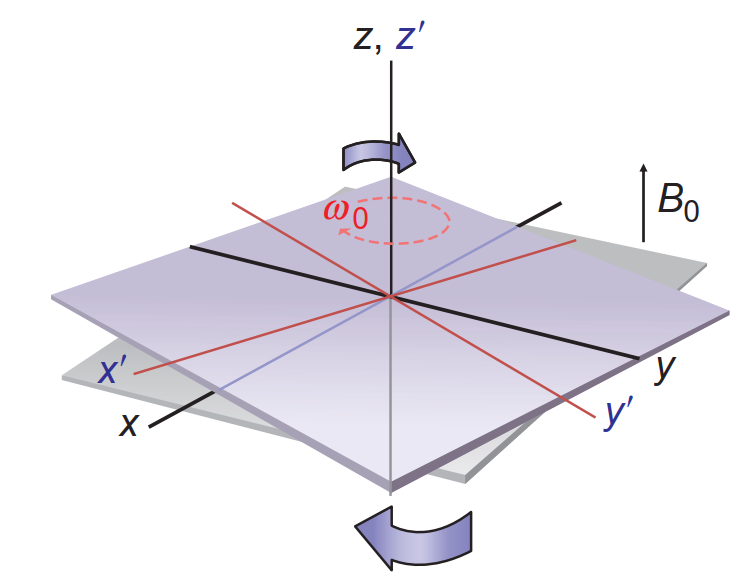
\includegraphics[width=0.3\linewidth]{chapters/chapter-2/figs/rotating-axis}
			\label{subfig:rotating-axis-x'oy'}
		}{\scriptsize\Doi{10.1017/9781107706958.010}}
	}
	\hfill
	\subfigure[]{
		\copyrightbox[b]{
			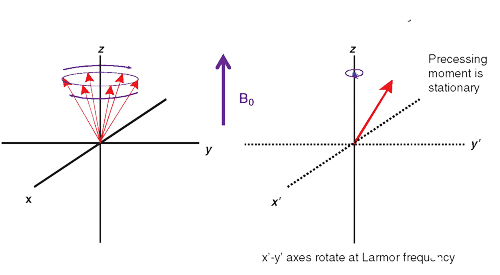
\includegraphics[width=0.6\linewidth]{chapters/chapter-2/figs/rotating-frame}
			\label{subfig:rotating-frame}
		}{\urlSource{musculoskeletalkey.com/magnetic-resonance-imaging-2/}}
	}
	\caption{}
	\label{fig:rotating-axis}
\end{figure}


سیگنال \lr{RF} یک سیگنال با پهنای باند بسیار باریک حول یک فرکانس مرکزی می‌باشد. در طی این فرایند، پروتون ها انرژی آن را در فرکانس مشخصی دریافت می‌کنند. با نوشتن روابط کوانتومی در 
 \cite{McRobbie}، 
 می‌توان نشان داد که رابطه این فرکانس خاص و میدان $B_0$ مجددا از تساوی لارمور در رابطه‌ی 
 \ref{eq:larmor}
  محاسبه می‌شود و این یعنی آن فرکانس خاص همان $\omega_0$ است. همچنین اختلاف دو سطح مذکور انرژی نیز از رابطه‌ی زیر بدست می‌آید که به معادله‌ی موج بروگلی
  \LTRfootnote{De Broglie’s wave equation}
   ناشی می‌شود.
  
  \removevspace
  \begin{align}
  	\Delta E = \hbar \omega_0 = (\frac{+1}2 - \frac{-1}2) \gamma \hbar B_0 = \gamma\hbar B_0
  \end{align}

که در آن $\hbar$ ثابت پلانک
\LTRfootnote{Planck's Constant}
با مقدار 
$\hbar = 6.62607004 \times 10^{-34} (\mathrm{m}^2 \mathrm{kg} / \mathrm{s})$
می‌باشد. بنابراین صرفا انرژی در این فرکانس $\omega_0$ پروتون را برمی‌انگیزد که از اسپین خود را تغییر دهند و بین سطوح انرژی جابجا شوند.
این انرژی کوانتیده به‌عنوان \textbf{انرژی جذب رزونانسی و یا تشدیدی}
\LTRfootnote{Resonance Absorption Energy} 
شناخته می‌شود و فرکانس مربوط به آن را \textbf{فرکانس تشدید}
\LTRfootnote{Resonant Rrequency}
می‌نامند. از این نکته می‌توان دلیل نام گذاری \mri و مخصوصا بخش رزونانسی آن را متوجه شد.


\begin{figure}[t!]
	\centering
	\copyrightbox[b]{
		\begin{minipage}{0.9\linewidth}\centering
			\begin{RTL}
			\subfigure[]{
				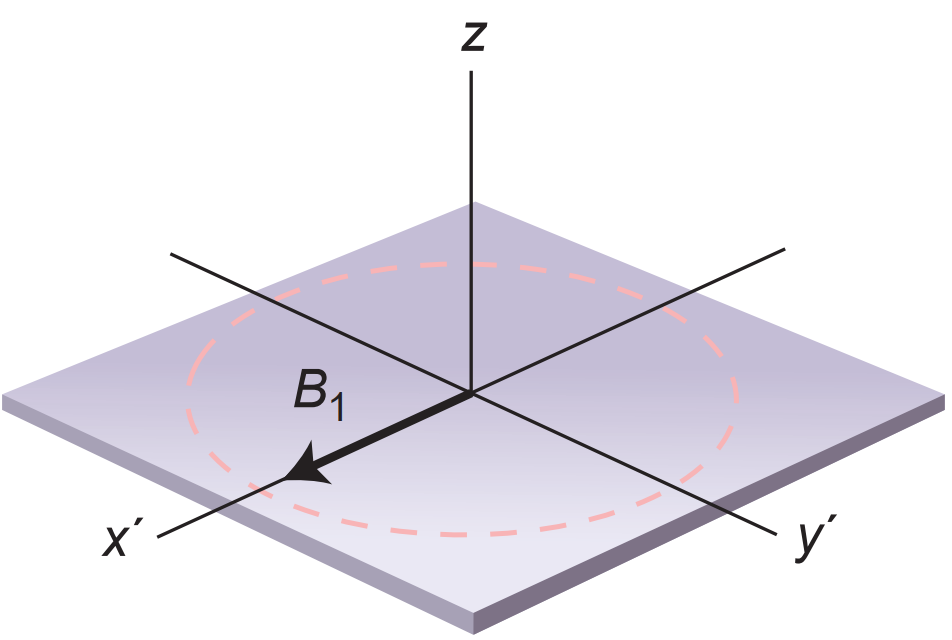
\includegraphics[width=0.25\linewidth]{chapters/chapter-2/figs/rot-a}\label{subfig:rot-a}}
			\hspace{0.075\linewidth}
			\subfigure[]{
				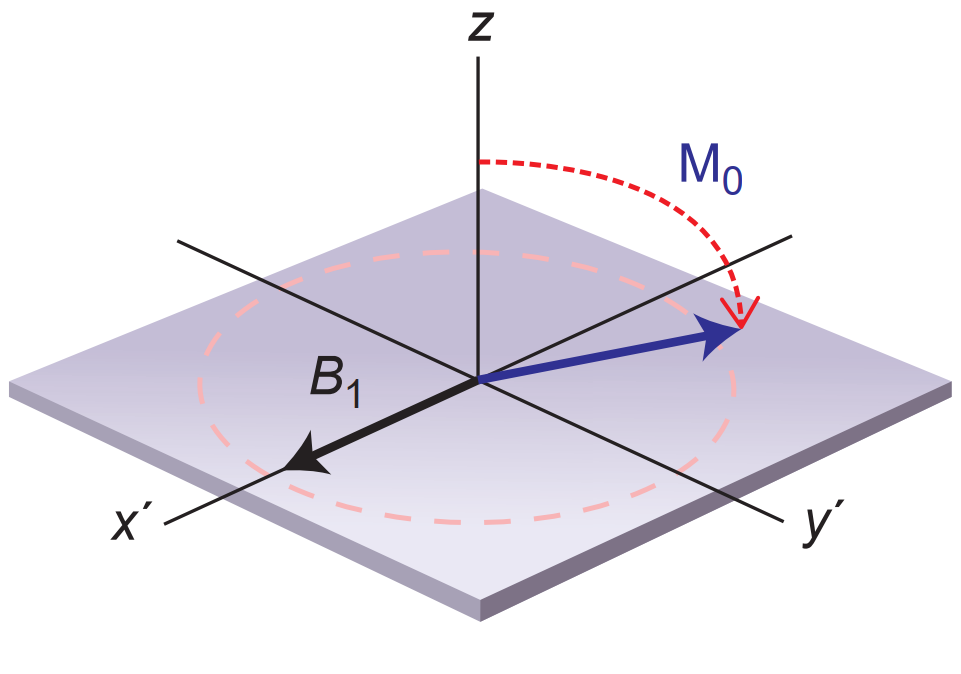
\includegraphics[width=0.25\linewidth]{chapters/chapter-2/figs/rot-b}\label{subfig:rot-b}}
			\hspace{0.075\linewidth}
			\subfigure[]{
				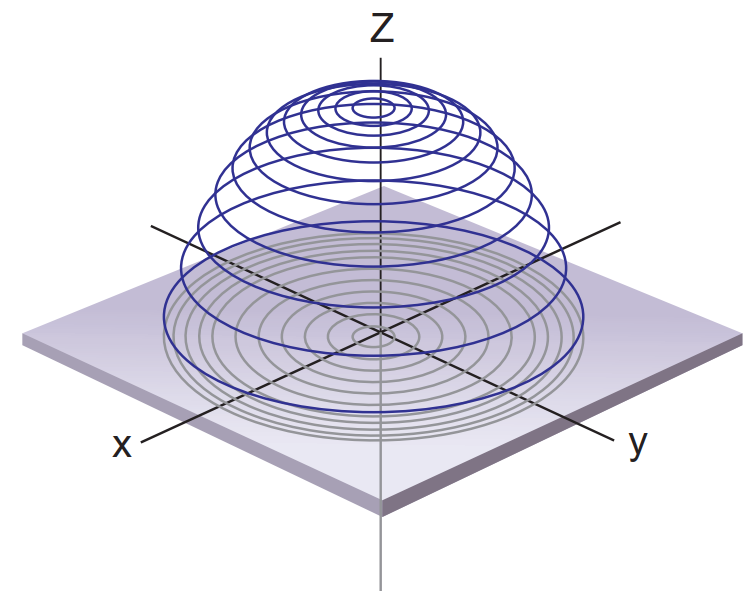
\includegraphics[width=0.25\linewidth]{chapters/chapter-2/figs/rot-c}\label{subfig:rot-c}}
			\end{RTL}
		\end{minipage}
	}{\scriptsize\Doi{10.1017/9781107706958.010}}
\end{figure}


\begin{figure}[t]
\centering
\begin{RTLcopyrightBox}{\linewidth}{\urlSource{http://hyperphysics.phy-astr.gsu.edu/hbase/phyopt/polclas.html}}
	\subfigure[]{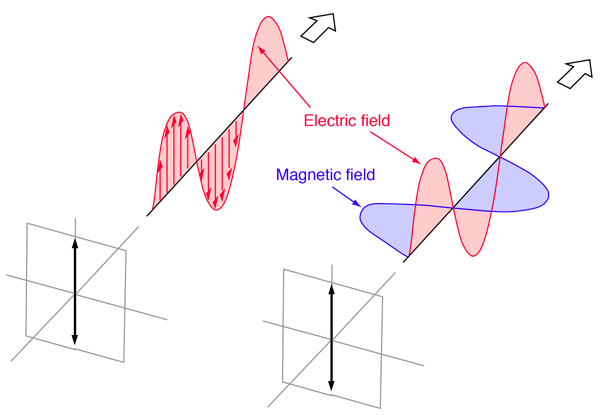
\includegraphics[height=0.26\linewidth]{chapters/chapter-2/figs/wave-linear-circular-pol}}
	\hfill
	\subfigure[]{
\includegraphics[height=0.26\linewidth]{chapters/chapter-2/figs/polcls}}
	\removevspace[1]
	\caption{}
\end{RTLcopyrightBox}
\label{fig:wave-linear-circular-pol}
\end{figure}
%\begin{figure}[t]
%	\centering
%	\copyrightbox[b]{
%		\includesvg[width=0.4\linewidth]{chapters/chapter-2/figs/Onde_electromagnetique.svg}\label{fig:Onde_electromagnetique.svg}
%	}{\urlSource{https://w.wiki/3svH}}
%\end{figure}

پالس \lr{RF} توسط یک سیم‌پیچ فرستنده که بر میدان $B_0$ عمود است، ایجاد می‌شود و یک میدان مغناطیسی  $B_1$ که عمود بر میدان $B_0$ و با فرکانس تشدید لارمور $\omega_0$ در حال نوسان است، را ایجاد می‌کند. بنابراین دیگر موله عرضی $M_0$ صفر نمی‌باشد. فرض کنید این میدان جدید $B_1$ 
در دستگاه گردان شکل \ref{eq:x'oy'}
در راستای $x'$ تعریف شده است. از آن‌جا که این میدان با فرکانس $\omega_0$ در حال نوسان است، در این دستگاه مختصات گردان به صورت ایستان ظاهر می‌شود 
(شکل \ref{subfig:rot-a})
و فرض است که میدان $B_0$ نیز در راستای محور $z$ ها تعریف شده است. این میدان جدید مغناطش شبکه ($M_0$)
را در طول زمان جابجا میکند. این جابجایی در دستگاه مختصات گردان، به شکل خیلی ساده حول محور $x'$ ها و با سرعت ثابت جابجا می‌شود(البته اگر میدان $B_1$ در طول زمان مقدار ثابتی داشته باشد) که در شکل \ref{subfig:rot-b}
این جابجایی را از محور $z$ تا محور $y'$ را نمایش می‌دهد. این جابجایی را می‌توان بر حسب زمان و براساس \textbf{زاویه‌ی تکان}
\LTRfootnote{Flip Angle}
 $\alpha$ به شکل زیر فرمول‌بندی کرد.

\removevspace
\begin{align}
	\alpha = \gamma B_1 t_p
\end{align}




که در آن $B_1$ اندازه‌ی میدان مغناطیسی سیگنال $RF$ است و $t_p$ طول زمان اعمال پالس است. اگر پالس \lr{RF} درست در زمانی که $M_0$ به صفحه‌ی مولفه‌‌ی عمودی برسد پایان بیابد، $\alpha=90\degree$ می‌شود و پالس \lr{RF} یک \textbf{پالس $90\degree$} نامیده می‌شود. اگر قدرت و یا طول مدت اعمال این سیگنال دوبرابر شود، بردار $M_0$ دقیقا $180\degree$ می‌چرخد و پالس متناظر با آن را \textbf{پالس $180\degree$} می‌نامند. 
\hl{بنابراین زمان اهمیت ویژه‌ای در اساس کار دستگاه‌های \mri دارد}
\cite{McRobbie}.
شکل \ref{subfig:rot-c}
مسیر حرکت بردار $M_0$ را در دستگاه مختصات معمول $xoy$ نشان می‌دهد که مسیری فنری را طی می‌کند.
همچنین پالس \lr{RF} یک اثر مهم دیگری که بر‌روی اسپین ها دارد این است که آن‌ها را هم‌فاز می‌کند. به عبارت‌ دیگر تمام آن ها در روی دایره ی گردان، به یک نقطه اشاره می‌کنند. شکل \ref{fig:rotating-axis-coil} خلاصه‌ای از آن‌چه که گفته شد را نشان می‌دهد.



 
 
 \begin{figure}
 	\centering
	\copyrightbox[b]{
	 	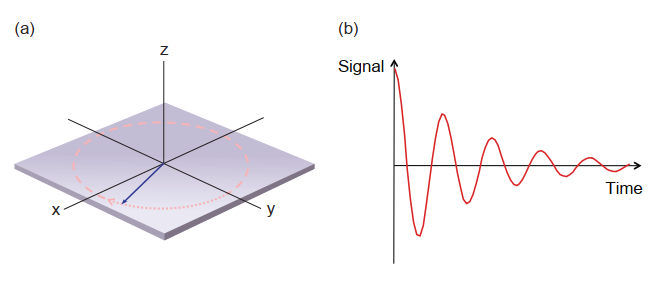
\includegraphics[width=0.8\linewidth]{chapters/chapter-2/figs/signal-recived}
	}{\scriptsize\Doi{10.1017/9781107706958.010}}
 	\caption{}
 	\label{fig:signal-recived}
 \end{figure}
 
 
 
 با جابجایی بردار $M_0$ به سمت صفحه‌ی عرضی و حرکت تقدیمی آن به دور محور $z$ ها یک میدان مغناطیسی نوسانی ایجاد می‌شود که می‌توان آن را توسط ولتاژی که روی یک سیم‌پیچ گیرنده القا می‌کند، اندازه گیری نمود. 
 این سیم‌پیچ صرفا به میدان های مغناطیسی عمود بر راستای $B_0$ حساس می‌باشد. بنابراین در این هنگام باید سیم پیچ فرستنده خاموش شود و در سیم پیچ گیرنده ولتاژی القا می‌شود که با فرکانس $\omega_0$ تغییر می‌کند. دامنه‌ی این ولتاژ القایی به صورت نمایی به سمت صفر تنها در عرض چند میلی ثانیه میرا می‌شود(شکل \ref{fig:signal-recived})
چرا که پروتون ها به سرعت نسبت به یک دیگر دیفاز 
\LTRfootnote{Dephase}
می‌شوند. این سیگنال \textbf{القای آزاد میرا‌شونده (\lr{FID})}
\LTRfootnote{Free Induction Decay} 
نامیده می‌شود\cite{JosephHornak}
 که در مورد آن بیشتر صحبت خواهد شد.

\subsection{سیگنال \lr{FID} و آزادسازی}

به محض آن‌که پالس \lr{RF} قطع می‌شود، پروتون هایی که بردار مغناطیسی آن ها به سمت صفحه عرضی متمایل شده بود، به نقطه تعادل خود باز گردند. در این \textbf{آزاد‌سازی} 
\LTRfootnote{Relaxation}
دو اتفاق اصلی می‌افتد:
\begin{enuminline}
	\item پروتون‌ها انرژی ای را که در فرکانس $\omega_0$ جذب کرده بودند را از خود منتشر می‌کنند.
	\item اسپین‌هایی که بعد از اعمال فاز هم‌فاز شده‌اند، فاز خود را از دست می‌دهند و مغناطش شبکه به محور $B_0$ باز می‌گردد و حول آن مانند یک ژیروسکوپ به حرکت تقدیمی می‌پردازد (شکل \ref{fig:rotating-axis-coil}).
\end{enuminline}




\begin{figure}
	\centering
	\copyrightbox[b]{
		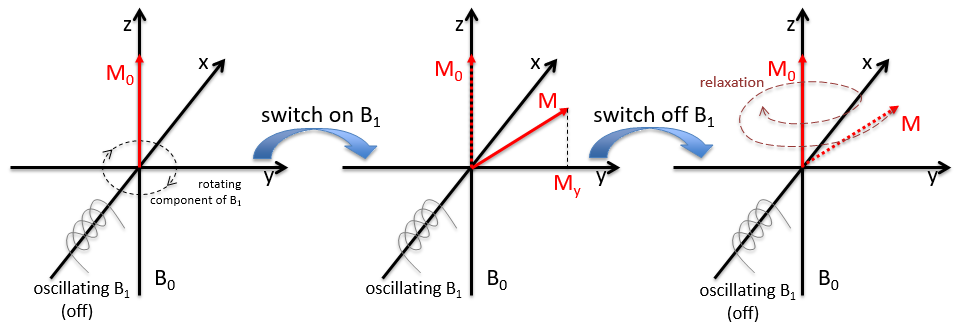
\includegraphics[width=0.9\linewidth]{chapters/chapter-2/figs/HRMN6}
	}{\urlSource{https://musculoskeletalkey.com/magnetic-resonance-imaging-2/}}
	\caption{}
	\label{fig:rotating-axis-coil}
\end{figure}

علت دیفاز شدن اسپین ها، اختلاف اندکی است که بین فرکانس تقدیمی آن ها وجود دارد. برای درک بهتر این موضوع، یک دستگاه مختصات گردان با فرکانس لارمور $\omega_0$ شکل \ref{eq:x'oy'} را در نظر بگیرید. اگر اسپینی فرکانس تقدیمی آن کمی بیشتر باشد، در جهت عقربه های ساعت و اگر کمی کمتر باشد، در خلاف جهت عقربه های ساعت دیفاز می‌شود. بنابراین هر چیزی که باعث تغییرات کمی در فرکانس  آن ها از فرکانس لارمور شود، منجر به دیفاز شدن آن می‌شود. \cite{McRobbie}

گفته شد که مولفه‌ی عرضی $M_0$ ولتاژی را موسوم به \lr{FID} در سیم پیچ های گیرنده القا می‌کند. به‌طور‌کلی، 
این سیگنال \lr{FID} سه مولفه‌ی مورد علاقه دارد: اندازه 
\LTRfootnote{Magnitute}
(پیک دامنه‌)، فرکانس و فاز (جهت نسبت به فاز سیگنال \lr{RF} فرستنده).
اندازه سیگنال متناسب به مقدار $M_0$ قبل از اعمال پالس \lr{RF} است. فرکانس آن نیز همان فرکانس لارمور در رابطه ی \ref{eq:larmor} است که با اندازه میدان مغناطیسی $B_0$ که پروتون ها تحت تاثیر آن هستند، متناسب است.
اگر تمام پروتون ها تحت تاثیر یک میدان مغناطیسی $B_0$ یکسان قرار داشته باشند،  بنابراین تنها یک فرکانس درون \lr{FID} دیده می‌شود. در واقعیت میدان مغناطیسی $B_0$ در سراسر بدن بیمار تغییر می‌کند. بنابراین سیگنال \lr{MR}
شامل چندین فرکانس  است که در طول زمان متناسب با سیگنال \lr{RF} تغییر می‌کند. ساده تر است که چنین سیگنال چند فرکانسی را در حوزه فرکانس بررسی کرد که این حوزه نیز با یک تبدیل فوریه 
\LTRfootnote{Fourier Transformation}
از حوزه زمان بدست می‌آید.\cite{book:basic-principles-and-applications}



\begin{figure}
	\centering
	\copyrightbox[b]{
	\begin{minipage}{\linewidth}\centering
	\subfigure[]{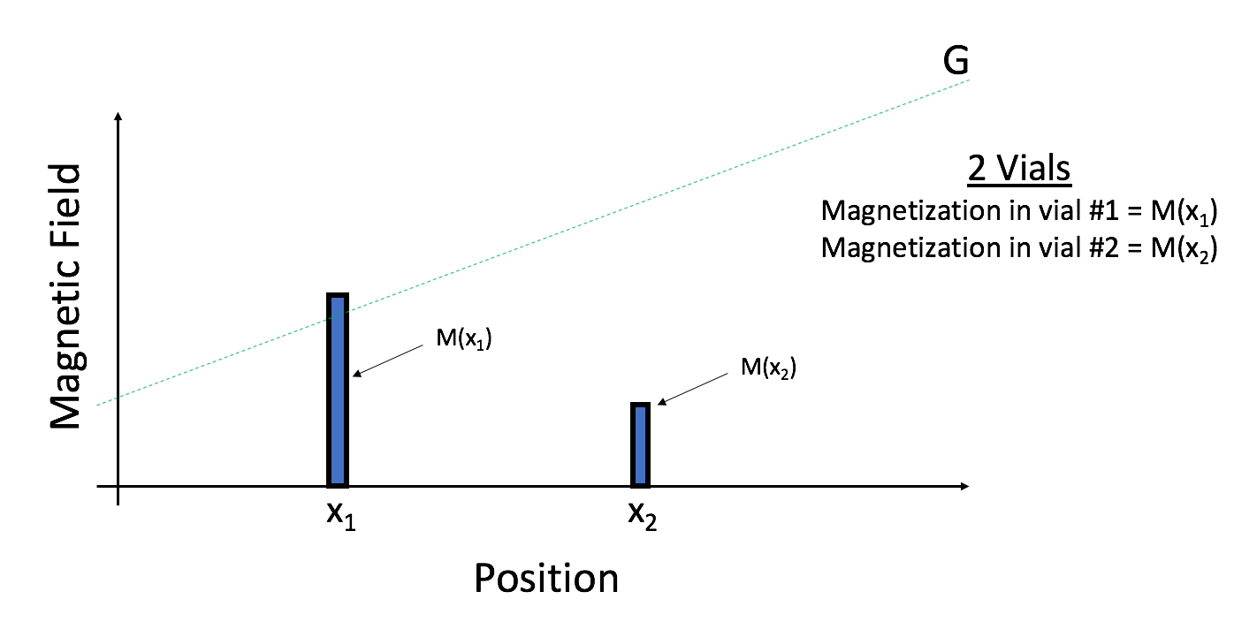
\includegraphics[height=0.23\linewidth]{chapters/chapter-2/figs/gr-1}\label{subfig:gr1}}
	\hspace{0.08\linewidth}
	\subfigure[]{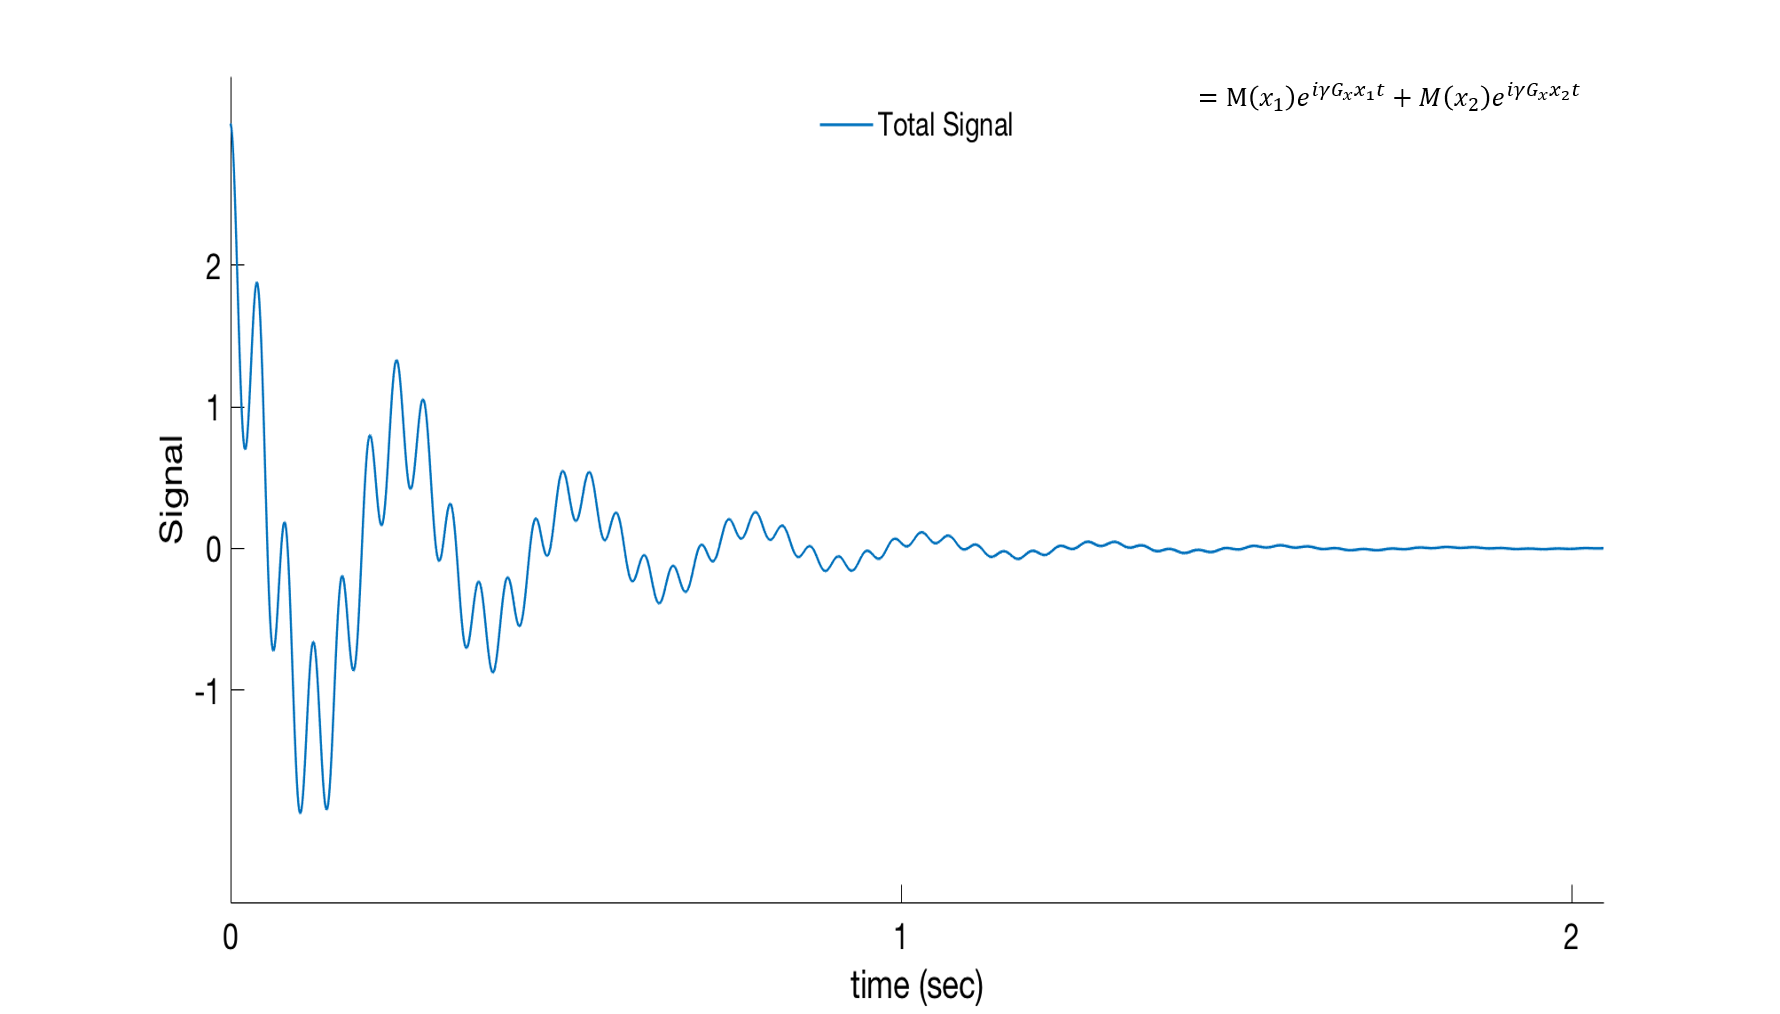
\includegraphics[height=0.23\linewidth]{chapters/chapter-2/figs/gr-3}\label{subfig:gr3}}
	\subfigure[]{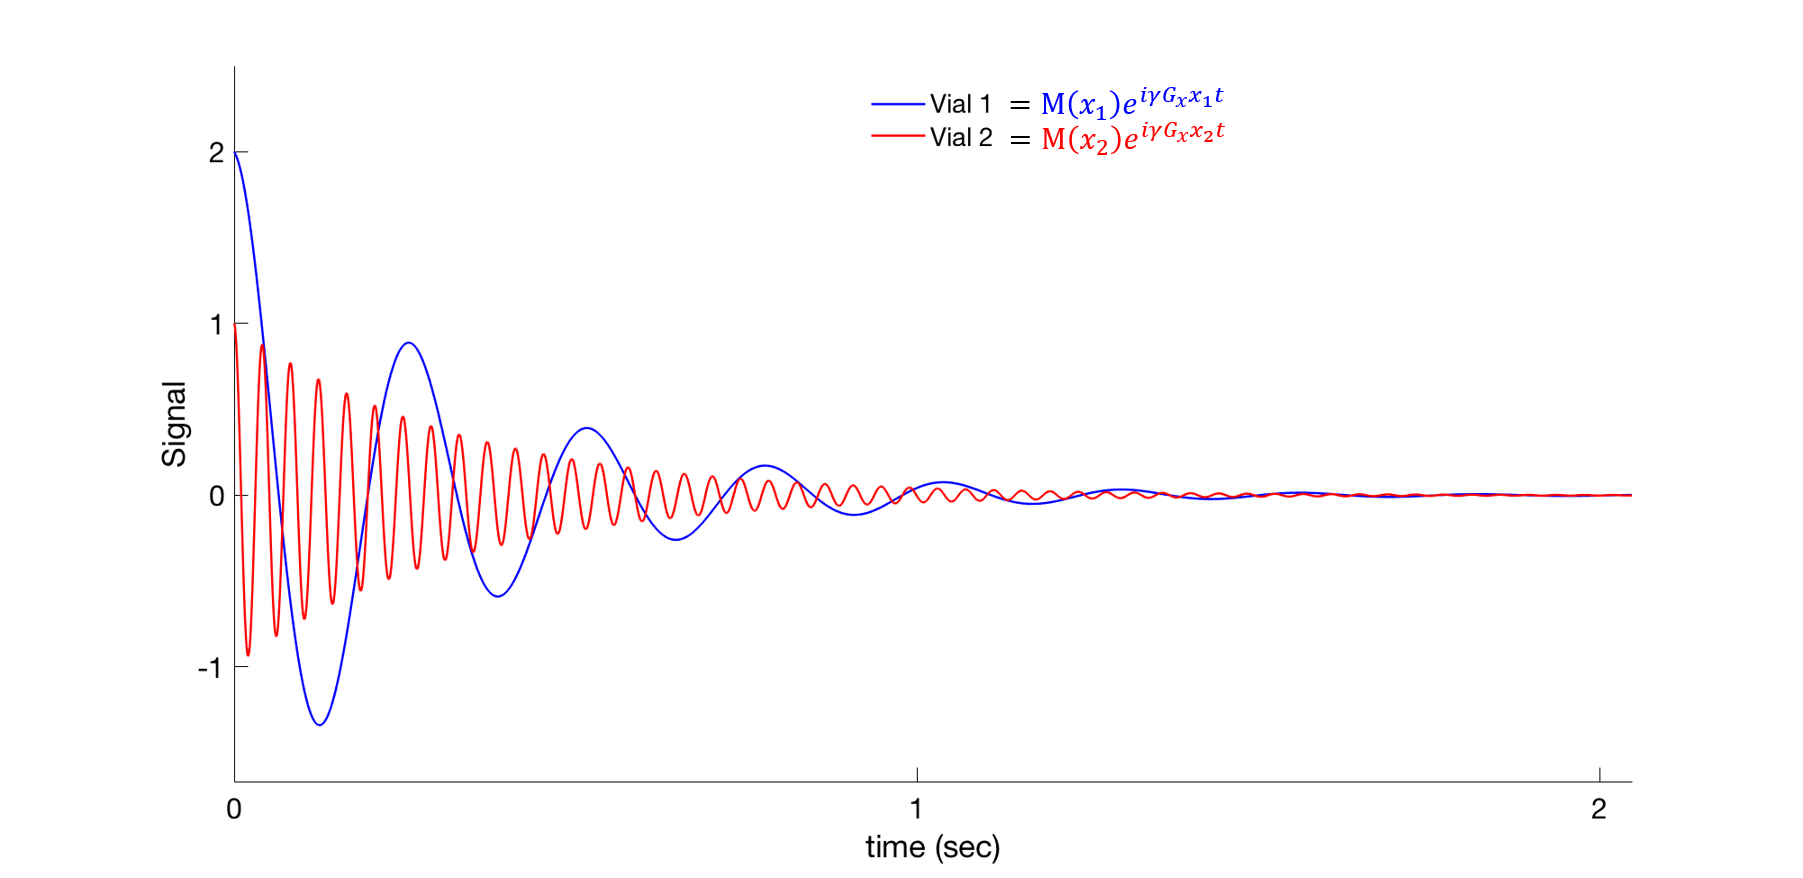
\includegraphics[height=0.23\linewidth]{chapters/chapter-2/figs/gr-2}\label{subfig:gr2}}
	\hspace{0.08\linewidth}
	\subfigure[]{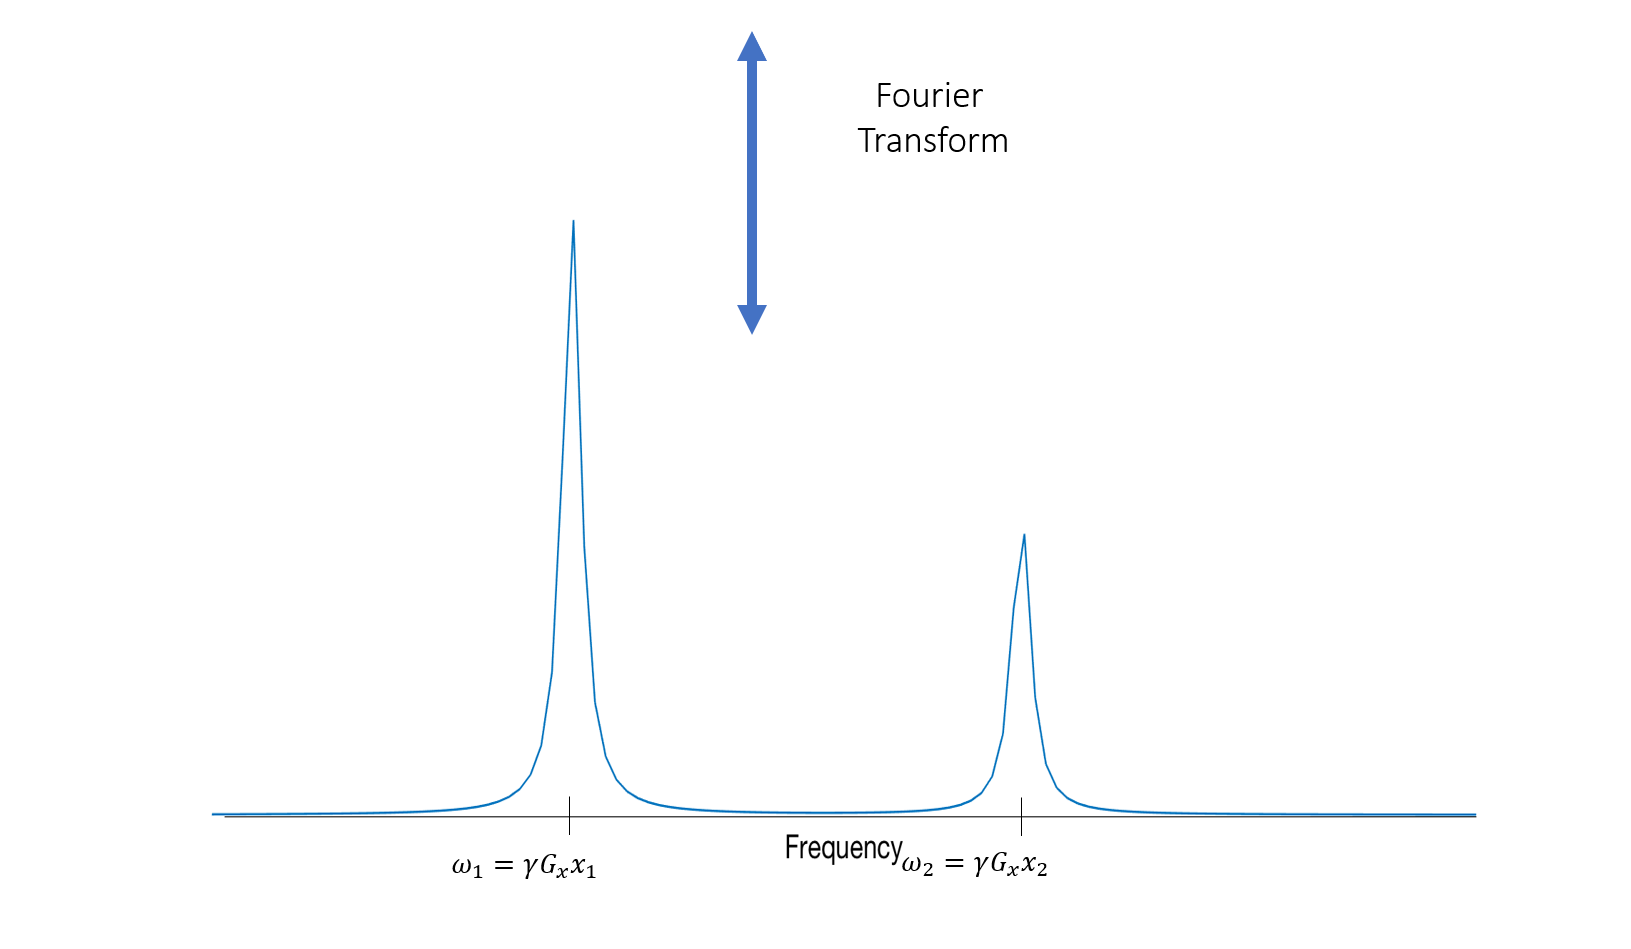
\includegraphics[height=0.25\linewidth]{chapters/chapter-2/figs/gr-4}\label{subfig:gr4}}
	\end{minipage}
	}{\urlSource{https://yout.be/vC82NeZmL-M}}
	\removevspace
	\caption{}
	\label{fig:gr}
\end{figure}


\begin{figure}[t!]
	\centering
	\copyrightbox[b]{
		\includegraphics[width=0.6\linewidth]{chapters/chapter-2/figs/sampling-freq.bmp}
	}{\scriptsize\Doi{10.1002/jmri.23639}}
	\caption{}
\end{figure}



\subsubsection{آزادسازی \lr{T1}}


\subsubsection{آزادسازی \lr{T2}}

%Selection of T1 and T2 values for tissues at 0.5 T, 1.5 T and 3 T. All values measured in vivo from human tissues
\begin{table}[b!]
	\centering
	\begin{latin}
		\begin{copyrightBox}{0.7\linewidth}{\scriptsize\Doi{10.1017/9781107706958.010}}
			\rowcolors{2}{gray!10}{white}
			\begin{tabular}{|c|ccc|ccc|}
				\hline \rowcolor{headerColor}
				& \multicolumn{3}{c|}{T1 (ms)} & \multicolumn{3}{c|}{T2 (ms)} \\
				\rowcolor{headerColor} Tissue & 0.5 T & 1.5 T & 3 T & 0.5 T & 1.5 T & 3 T \\\hline\hline
				White matter & 520 & 560 & 832 & 107 & 82 & 110 \\
				Grey matter & 780 & 1100 & 1331 & 110 & 92 & 80 \\
				CSF  & –  & 2060 & 3700 & – & – & – \\
				Muscle & 560 & 1075 & 898 & 34 & 33 & 29 \\
				Fat & 192 & 200 & 382 & 108 & – & 68 \\
				Liver & 395 & 570 & 809 & 96 & – & 34 \\
				Spleen & 760 & 1025 & 1328 & 140 & – & 61 \\\hline
			\end{tabular}
		\end{copyrightBox}
	\end{latin}
	\removevspace[1.]
	\caption{}
\end{table}



\begin{figure}[t!]
	\centering
	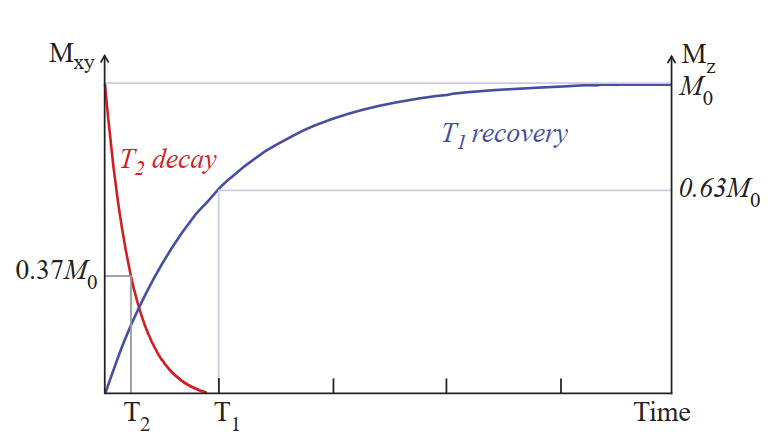
\includegraphics[width=0.5\linewidth]{chapters/chapter-2/figs/t1-t2-ralaxation-time}
	\removevspace
	\caption{}
	\label{fig:t1-t2-ralaxation-time}
\end{figure}

\subsubsection{اسپین-اکو}

\begin{figure}[t!]
	\centering
	\subfigure[]{
	\copyrightbox[b]{
		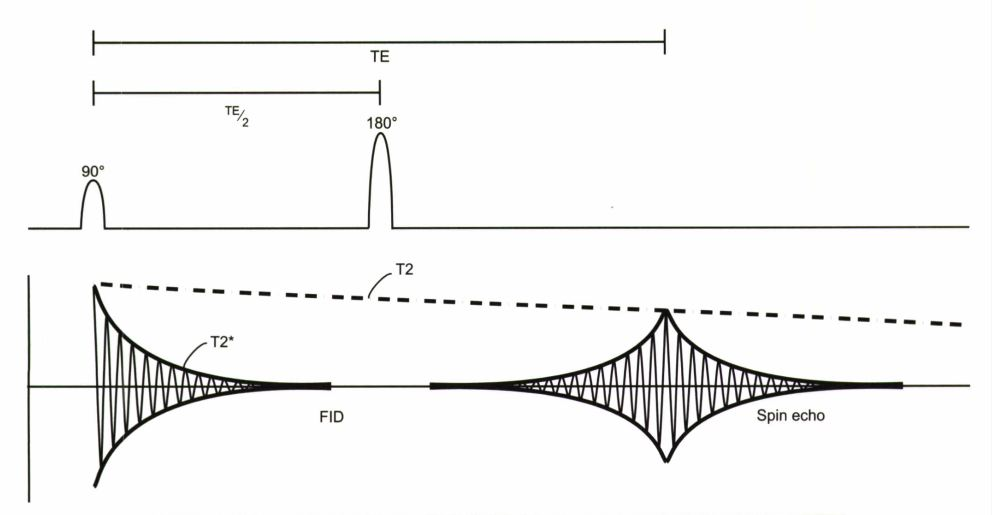
\includegraphics[width=0.5\linewidth]{chapters/chapter-2/figs/spin-echo}
	}{\urlSource{https://is.gd/rSpAtw}}}
	\hfill
	\subfigure[]{
	\copyrightbox[b]{
		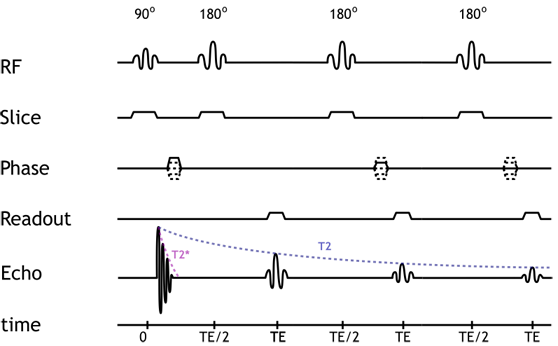
\includegraphics[width=0.45\linewidth]{chapters/chapter-2/figs/fse_diag}
	}{\urlSource{http://xrayphysics.com/sequences.html}}}
	\caption{}
	\label{fig:spin-echo}
\end{figure}



\subsection{گرادیان}


\begin{figure}[t!]
	\centering
	\begin{RTLcopyrightBox}{\linewidth}{\urlSource{http://mriquestions.com/gradient-coils.html}}
		\subfigure[]{
			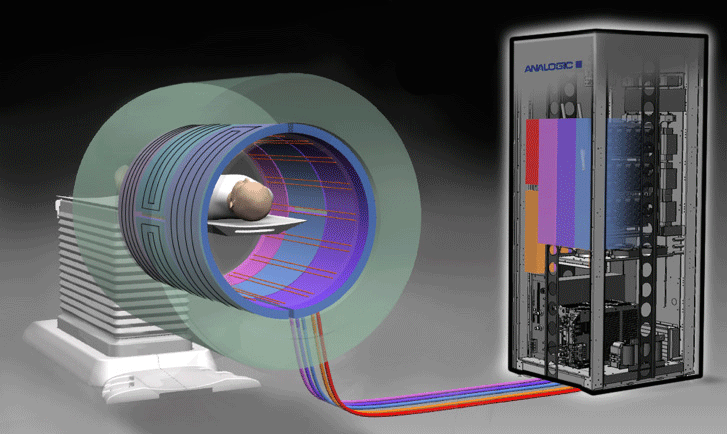
\includegraphics[height=0.27\linewidth]{chapters/chapter-2/figs/gradinent-coil-real}
			\label{subfig:gradinent-coil-real}}
		\subfigure[]{
			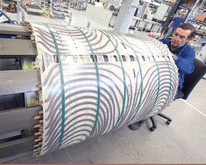
\includegraphics[height=0.27\linewidth]{chapters/chapter-2/figs/gradinent-coil-guy}
			\label{subfig:gradinent-coil-guy}}
		\subfigure[]{
			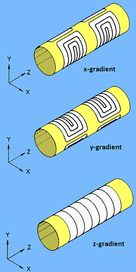
\includegraphics[height=0.27\linewidth]{chapters/chapter-2/figs/gradinent-coil}
			\label{subfig:gradinent-coil}}
	\end{RTLcopyrightBox}
	\removevspace
	\caption{}
\end{figure}%https://www.cis.rit.edu/htbooks/mri/chap-9/chap-9-h5.htm




\sidecaptionvpos{figure}{b}
\begin{SCfigure}[1.5][t!]
	\centering
	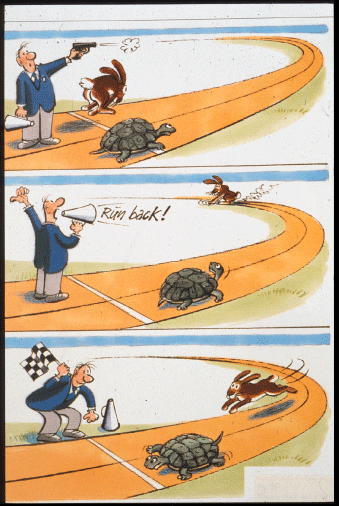
\includegraphics[width=0.3\linewidth]{chapters/chapter-2/figs/tortoise_hare-gre}
	\caption[دوندگان در یک مسیر]{دوندگان در یک مسیر.}
	\label{fig:tortoise-hare-gre}
\end{SCfigure}





\begin{figure}[t!]
	\centering
	\copyrightbox[b]{
		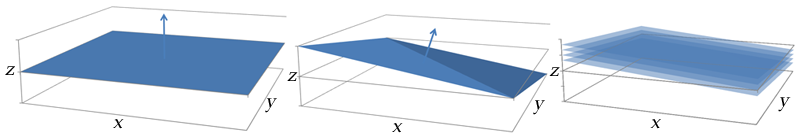
\includegraphics[width=0.7\linewidth]{chapters/chapter-2/figs/oblique_grad}
	}{\urlSource{http://xrayphysics.com/spatial.html}}
	\removevspace[1]
	\caption{}
	\label{fig:obliquegrad}
\end{figure}













\begin{figure}
	\centering
	\subfigure[]{
	\copyrightbox[b]{
		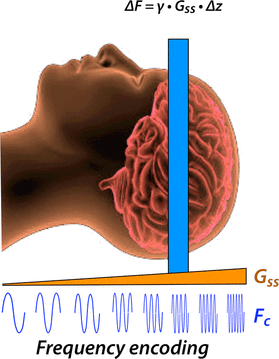
\includegraphics[width=0.2\linewidth]{chapters/chapter-2/figs/Slice-selection-freq-enc}
	}{\lr{\scriptsize source: \urlWithoutHttps{is.gd/1adUOy}}}}
	\hfill
	\subfigure[]{
		\copyrightbox[b]{
			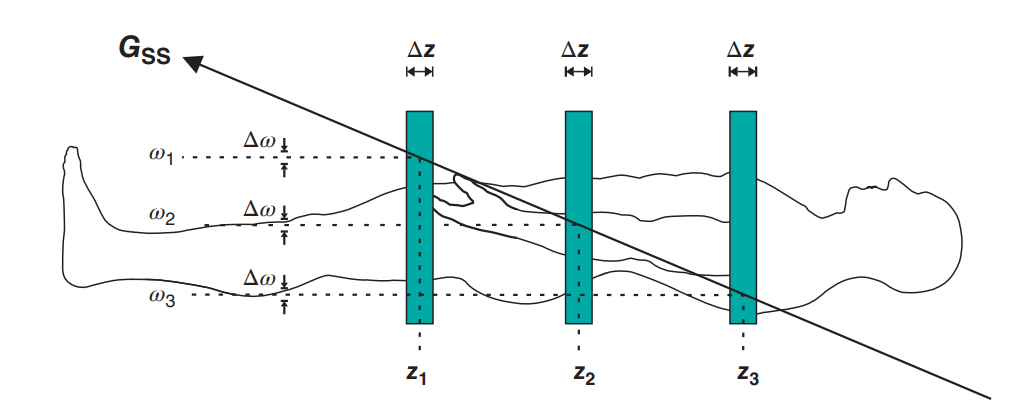
\includegraphics[width=0.7\linewidth]{chapters/chapter-2/figs/Slice-selection-process}
		}{\scriptsize\Doi{10.1002/9781119013068}}}


	\caption{}
	\label{fig:slice-selection-process}
\end{figure}

\begin{figure}[t!]
	\centering
	\copyrightbox[b]{
		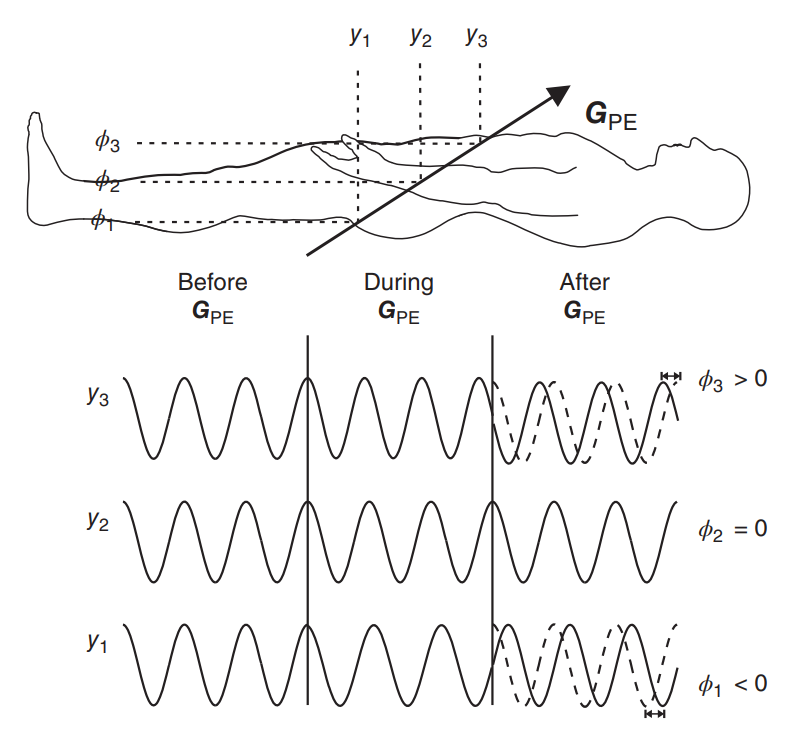
\includegraphics[width=0.7\linewidth]{chapters/chapter-2/figs/Concept-of-phase-encoding}
	}{\scriptsize\Doi{10.1002/9781119013068}}
	\caption{}
	\label{fig:concept-of-phase-encoding}
\end{figure}


\begin{figure}[t!]
	\centering
	\copyrightbox[b]{
		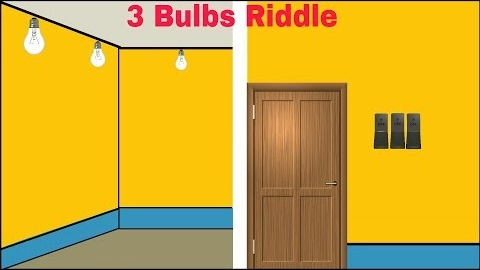
\includegraphics[width=0.4\linewidth]{chapters/chapter-2/figs/3switches-3bulbs}
	}{\urlSource{http://youtu.be/bN_ra_PYS2o}} %https://img.youtube.com/vi/bN_ra_PYS2o/0.jpg
%	\copyrightbox[b]{
%		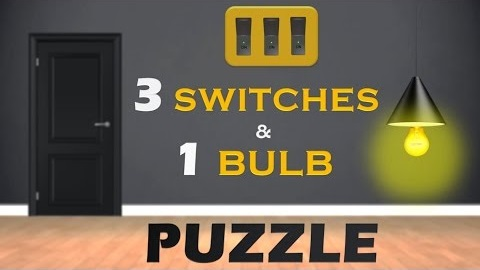
\includegraphics[width=0.4\linewidth]{chapters/chapter-2/figs/3switches-one-bulb}
%	}{\urlSource{http://youtu.be/w22pXPMUow0}}
	\removevspace[1]
	\caption{معمای سه کلید و سه لامپ}
	\label{fig:3switches-3bulbs}
\end{figure}

\FloatBarrier
\subsection{\kspace}


\begin{figure}[t!]
	\centering
	\copyrightbox[b]{
		\includegraphics[width=0.7\linewidth]{chapters/chapter-2/figs/kspace.bmp}
	}{\scriptsize\Doi{10.1002/jmri.23639}}
\end{figure}



\subsubsection{رزولوشن و میدان دید}


\begin{figure}[t!]
	\centering
	\begin{copyrightBox}{0.8\linewidth}{\scriptsize\Doi{10.1017/9781107706958}}
		\subfigure[]{
			\includegraphics[width=0.45\linewidth]{chapters/chapter-3/figs/kFOV-Dk}
			\label{subfig:kfov-dk}}
		\hfill
		\subfigure[]{
			\includegraphics[width=0.375\linewidth]{chapters/chapter-3/figs/FOV-Dw}
			\label{subfig:fov-dw}}
	\end{copyrightBox}
	\removevspace[1]
	\caption{}
\end{figure}



\removevspace
\begin{subequations}\label{eq:FOV-kFOV}
\begin{align}
	\Delta k = & \dfrac{1}{\rltext{FOV}} \\
	 k\rltext{FOV}_w = & (+k_{w,\max}) - (-k_{w,\max}) = 2 k_{w,\max} \\
	 = & N / \lrtext{FOV} = 1 / \Delta w
\end{align}
\end{subequations}

بیشسنه مقدار رزولوشن به وسیله‌ی اندازه‌ی پیکسل ها داده می‌شود که برابر است با:

\removevspace
\begin{subequations}
\begin{align}
\Delta x &= \dfrac{1}{\gammabar . G_\mathrm{FE} . M . \Delta t} \\ 
\Delta y &= \dfrac{1}{\gammabar . \Delta G . N . \tau}
\end{align}
\end{subequations}


اندازه ابعاد تصویر یا همان میدان دید (\lr{FOV})
نیز از رابطه‌ی  \ref{eq:FOV-kFOV}
به صورت زیر محاسبه می‌شود.

\removevspace
\begin{subequations}\label{eq:fov-res-kspace}
\begin{align}
	\lrtext{FOV}_{\mathrm{FE}} &= M . \Delta x = \dfrac{1}{\gammabar . G_\mathrm{FE} . \Delta t} \\ 
	\lrtext{FOV}_{\mathrm{PE}} &= N . \Delta y = \dfrac{1}{\gammabar . \Delta G . \tau} \\
	k\lrtext{FOV}_{\mathrm{FE}} &= M . \Delta k_x = 2 k_{x, \max} = \frac{1}{\Delta x}\\
	k\lrtext{FOV}_{\mathrm{PE}} &= N . \Delta k_y = 2 k_{y, \max} = \frac{1}{\Delta y}
\end{align}
\end{subequations}

\FloatBarrier
\subsubsection{ارتباط \kspace با کد کردن فرکانس و فاز}
پس از تحریک کردن یک اسلایس، گرادیان های فاز و فرکانس اعمال می‌شود تا سیگنال های \mr را جهت بدست آوردن فرکانس های فضایی بکار بگیریم. برای این منظور ابتدا، المان  $\partial s$  از سیگنال را در نظر بگیرید. 

\removevspace
\begin{equation}\label{eq:element-fe}
	\mathbf{\partial} s(t) = \rho(x) . \exp(\frac{-t}{T_2^*}) .  \exp(i\gamma.x.G_{\lrtext{FE}}.t). \mathrm{d}x
\end{equation}

در این رابطه $\rho(x)$
چگالی پروتون ها در راستای $x$ است. گرادیان $G_{\lrtext{FE}}$ به صورت پیوسته در جهت $x$ , در زمان نمونه برداری سیگنال $(t)$ اعمال می‌شود.گرادیان ناهمفاز کننده معمولا قبل از نمونه بردای اعمال می‌شود تا اکوی متقارنی ایجاد شود.

حال در جهت $y$ فاز را کد می‌کنیم. این کار با اعمال یک گرادیان $G_{\lrtext{PE}}$
به مدت زمان $\tau$ قبل از زمان نمونه برداری، انجام می‌پذیرد. یک المان کوچک از سیگنال $\partial s$ با اعمال هردو گرادیان به شکل زیر است.


\removevspace
 \begin{equation}\label{eq:element-fe-pe}
 		\mathbf{\partial} s(t) = \rho(x,y) . \exp(\frac{-t}{T_2^*}) .  \exp(i\gamma.x.G_{\lrtext{FE}}.t).  \exp(i\gamma.y.G_{\lrtext{PE}}.\tau). \mathrm{d}x \mathrm{d}y
 \end{equation}


به عبارت دیگر

\removevspace
\begin{equation*}
	\rltext{سیگنال} = \rltext{چگالی اسپین ها} \times \rltext{میرایی \TtwoStar} \times \rltext{تغییر فاز ناشی از $G_{\lrtext{FE}}$ } \times \rltext{تغییر فاز ناشی از $G_{\lrtext{PE}}$ }
\end{equation*}


سیگنال نهایی از انتگرال المان فوق نسبت به $x$ و $y$ حاصل می‌شود:

\removevspace
\begin{subequations}\label{eq:iint-element-fe-pe}
\begin{align}
	S(t, \tau) =& \int \partial s(t) \\
	=& \iint \rho(x,y) . \exp(\frac{-t}{T_2^*}) .  \exp(i\gamma.x.G_{\lrtext{FE}}.t).  \exp(i\gamma.y.G_{\lrtext{PE}}.\tau). \mathrm{d}x \mathrm{d}y
\end{align}
\end{subequations}

در معادله \ref{eq:iint-element-fe-pe} مفهوم زمان های $t$ و $\tau$ به صورت پیوسته آمده است، این در حالی است که از سیگنال $M$ بار در بازه های $\Delta t$ نمونه برداری و هر سری پالس نیز $N$ مرتبه تکرار  شده است که در هر مرحله از آن، دامنه گرادیان $G_{\lrtext{PE}}$ افزایش یافته است:

\removevspace
\begin{equation} \label{eq:def-gpe}
	G_{\lrtext{PE}} = \Delta G . n \qquad  : \quad n = -\left(\frac{N}{2}\right) \rltext{تا} \left(\frac{N}{2} - 1\right)
\end{equation}
 
 در داخل نمایی های تغییرات فاز معادله \ref{eq:iint-element-fe-pe} را نیز می‌‌توان با تعریف
  $k_{\lrtext{FE}}$
و 
$k_{\lrtext{PE}}$
به صورت زیر، ساده‌تر نمود.

\removevspace
\begin{subequations} \label{eq:def-kpe-kfe}
\begin{align}
	k_{\lrtext{FE}} &= \gammabar . G_{\lrtext{FE}} . \Delta t . m \\
	k_{\lrtext{PE}} &= \gammabar . \Delta G . n . \tau
\end{align}
\end{subequations}

حال با در نظر گرفتن معادلات \ref{eq:def-kpe-kfe} و \ref{eq:def-gpe}، 
می‌توان نسخه گسسته معادله \ref{eq:iint-element-fe-pe}
را به شیوه زیر باز نویسی نمود.

\removevspace
\begin{equation}\label{eq:rel-dft-kspace}
	S(m,n) = \iint \rho(x,y) . \exp(\frac{-t}{T_2^*}) .  \exp(i2\pi.x.k_{\lrtext{FE}}).  \exp(i2\pi.y.k_{\lrtext{PE}}). \mathrm{d}x \mathrm{d}y
\end{equation}
 
که در آن مطابق معادله \ref{eq:def-kpe-kfe}، $k_{\lrtext{FE}}$ تابعی از $m$ و $k_{\lrtext{PE}}$ تابعی از $n$ می باشد. اگر به معادله \ref{eq:rel-dft-kspace} دقیق تر بنگریم، مشاهده می‌کنیم اگر جمله $\exp(\frac{-t}{T_2^*})$ را در نظر نگیریم، به معکوس تبدیل فوریه چگالی اسپین می‌رسیم. بنابراین می‌توان نوشت:

\removevspace
\begin{equation} \label{eq:dft-rho}
		S(m,n) = \F\left[\rho(x,y)\right](k_{\lrtext{FE}}, k_{\lrtext{PE}})
\end{equation}

بنابراین $k$ در رابطه \ref{eq:def-kpe-kfe} همان فرکانس های فضایی مدنظر هستند و وجه تسمیه \kspace نیز همین موضوع است. البته توجه داشته باشید که معادله \ref{eq:dft-rho} کاملا صحیح نمی‌باشد چرا که از جمله میراشونده با نرخ \TtwoStar در معادله \ref{eq:rel-dft-kspace} صرف نظر شده است. این جمله در برخی از فرکانس ها بیشتر از دیگر فرکانس ها تاثیر می‌گذارد و در صورت عدم حذف آن می‌تواند باعث محوشدگی و کاهش رزولوشن تصویر شود.











\FloatBarrier
\subsection{مطالعه بیشتر}
منابع متعددی در زمینه \mri منتشر شده است. اما از نظر نویسنده این پایان‌نامه، مقالات \cite{McRobbie} و \cite{SpinEchoMagnetic2013} نگاه نسبتا پوشایی به فیزیک ابتدایی \mri دارند. همچنین از کتب \cite{book:basic-principles-and-applications} و \cite{book:MRIfromPictureToProton} نیز در نوشتن این مطالب استفاده شده‌است که منابع بسیار مفیدی در این زمینه هستند.

 همچنین از سایت های
 \url{http://xrayphysics.com/} و
 \url{http://mriquestions.com/}
 به عنوان مراجع آنلاین این پژوهش نام برد. کورسی نیز در کورسرا
 \LTRfootnote{\url{https://www.coursera.org/learn/mri-fundamentals}}
گذرانده شد. هرچند این کورس ناقص است اما به پیوستگی مطالب هنگام نوشتن مطالب کمک کرده است.


\FloatBarrier
\section{یادگیری عمیق}\label{ch:background|sec:deep-learning}













\begin{figure}
	\centering
	\copyrightbox[b]{
		\includegraphics[width=0.6\linewidth]{chapters/chapter-2/figs/deeplearning-mlp}
	}{\doiSource{10.1117/12.882726}}
	\removevspace[1]
	\caption{}
	\label{fig:deeplearning-mlp}
\end{figure}




\begin{figure}
	\centering
	\copyrightbox[b]{
		\includegraphics[width=0.6\linewidth]{chapters/chapter-2/figs/deeplearning-ae}
	}{\urlSource{https://towardsdatascience.com/1c083af4d798}}
	\removevspace[1]
	\caption{}
	\label{fig:deeplearning-ae}
\end{figure}









\begin{figure}
	\centering
	\copyrightbox[b]{
		\includegraphics[width=0.5\linewidth]{chapters/chapter-2/figs/deeplearning-skip-connection}
	}{\urlSource{https://theaisummer.com/skip-connections/}}
	\removevspace[1]
	\caption{}
	\label{fig:deeplearning-skip-connection}
\end{figure}




\begin{figure}
	\centering
	\copyrightbox[b]{
		\includegraphics[width=0.85\linewidth]{chapters/chapter-2/figs/deeplearning-unet}
	}{\urlSource{https://is.gd/cXwc4s}}
	\removevspace[1]
	\caption{}
	\label{fig:deeplearning-unet}
\end{figure}



\FloatBarrier
\section{حسگری فشرده}\label{ch:background|sec:compresed-sensing}



\begin{figure}[t!]
	\centering
	\includegraphics[width=0.7\linewidth]{chapters/chapter-2/figs/compressed-sensig-general-settings}
	\caption{}
	\label{fig:compressed-sensig-general-settings}
\end{figure}



\begin{equation}
	\mathbf{y}_{m\times1} = \mathbf{\Phi}_{m\times n} . \mathbf{x}_{n\times1} + \mathbf{w}_{m\times1}
\end{equation}

\[x_{n\times1} = \lrtext{k-sparse}\]







\chapter{مرورادبیات}\label{ch:literature-review}

\section{یادگیری عمیق}\label{ch:literature-review|sec:deep-learning}





\begin{figure}
	\centering
	\subfigure[]{\includegraphics[width=0.4\linewidth]{chapters/chapter-3/figs/deep-learning_a}}
	\hspace{0.1\linewidth}
	\subfigure[]{\includegraphics[width=0.4\linewidth]{chapters/chapter-3/figs/deep-learning_b}}
	\subfigure[]{\includegraphics[width=0.4\linewidth]{chapters/chapter-3/figs/deep-learning_c}\label{subfig:deep-learning-c}}
	\hspace{0.1\linewidth}
	\subfigure[]{\includegraphics[width=0.4\linewidth]{chapters/chapter-3/figs/deep-learning_d}}
	\caption{}
	\label{fig:deep-learning-model}
\end{figure}


در ساختار \lr{CS-MRI} تلاش می‌شود که مسيله‌ی بهینه سازی زیر حل شود تا از اسپارسیتی در یک حوزه تبدیل بتوان به منظور بازسازی تصویر از روی نقاط باقیمانده کند. مشکل اصلی این کار که در مقاله \cite{Lustig_2007} راه حل حسگری فشرده آن مورد بررسی قرار گرفت، این است که به بخاطر مفهوم مطلوب ناهمدوستی
\LTRfootnote{Incoherency}
مجبور به آپدیت کرد بین هردو حوزه‌ی تصویر و حوزه \kspace است.

\removevspace
\begin{subequations}
	\begin{align}
		\min_{\hat{z}\in\mathbb{C}^N} \ \ &\|\mathcal{T}z\|_1 \\
		\lrtext{s.t.} \ \ & \Rho_\Lambda([\hat{x}]) = \Rho_\Lambda([\hat{z}])
	\end{align}
\end{subequations}


مقاله \cite{Jin_2016}
توانست نشان دهد که بین اسپارسیتی در یک حوزه تبدیل از تصویر (یا
\lr{FRI}\LTRfootnote{Finite Rate Inovation})
و حوزه \kspace ارتباطی وجود دارد و این ارتباط به رنک پایین بودن
\LTRfootnote{Low-Rankness}
ماتریس ساختاریافته هنکل
\LTRfootnote{Structured Hankel Matrix}
در حوزه \kspace بر میگردد. به عبارت دیگر اگر سیگنال ورودی یک سیگنال \lr{FRI} باشد، ماتریس ساختار یافته هنکل آن در حوزه فوریه، رنک پایین خواهد بود.

بنابراین مسیله‌ی \lr{CS-MRI}
را می‌توان به شکل زیر در آورد که در \cite{Jin_2016} از آن به نام \lr{ALOHA} یاد برده است.



\removevspace
\begin{subequations}
	\begin{align}
		\min_{\hat{z}\in\mathbb{C}^N} \ &\mathrm{Rank}(\mathcal{H}_d(\hat{z})) \\
		\lrtext{s.t.} \ & \Rho_\Lambda([\hat{x}]) = \Rho_\Lambda([\hat{z}])
	\end{align}
\end{subequations}


حال میخواهیم این مسيله را به یک مسیله یادگیری عمیق 
\LTRfootnote{Deep-Learning}
تبدیل کنیم. از آنجایی که ما از ساختار شکل \ref{subfig:deep-learning-c}
استفاده می‌کنیم، مساعد است که یک تابع هزینه را روی حوزه تصویر تشکیل دهیم از این رو الگوریتم \lr{ALOHA} را به شکل زیر ویرایش می‌کنیم.


\begin{subequations}\label{eq:aloha-modify1}
	\begin{align}
		\min_{\hat{z}\in\mathbb{C}^N} \ \  & \| x - \F^{-1}{\hat{z}}\| \\
		\lrtext{s.t.} \ \  & \mathrm{Rank}(\mathcal{H}_d(\hat{z})) = s, \\
		& \Rho_\Lambda([\hat{x}]) = \Rho_\Lambda([\hat{z}])
	\end{align}
\end{subequations}

که در آن $s$ یک تخمینی از رنک ماتریس ساختار یافته هنکل است. توجه داریم که تابع
$\mathrm{Rank}(.)$
یک قید غیر کانوکس 
\LTRfootnote{non-convex}
است. در مقاله \cite{Jin_2016}
به پیشنهاد از روش تکمیل ماتریس 
\cite{Cand_s_2009}
استفاده از رنک هسته‌ای
\LTRfootnote{nuclear norm}
را برای حل این مشکل توصیه کرده است اما این مقاله روش دیگری را برای غلبه بر این مشکل را اتخاذ کرده است. 

در ابتدا از اعداد مختلط خود را خلاص می‌کنیم. این کار به سادگی با تعریف اپراتور $\Re(z): \mathbb{C}\rightarrow\mathbb{R}^2$
روبرو امکان پذیر است:
$\Re(z) = [\mathcal{Re}(z) \mathcal{Im}(z)]$

در این صورت می‌توان معادله \ref{eq:aloha-modify1}
را به صورت زیر با نویسی نمود.

\begin{subequations}
	\begin{align}
		\min_{\hat{z}\in\mathbb{C}^N} \ \  & \| x - \F^{-1}{\hat{z}}\| \\
		\lrtext{s.t.} \ \  & \mathrm{Rank}(\mathcal{H}_{d|2}(\Re(\hat{z}))) = Q \le 2s, \\ 
		& \Rho_\Lambda([\hat{x}]) = \Rho_\Lambda([\hat{z}])
	\end{align}
\end{subequations}

حال می خواهیم آن را به فرم یادگیری عمیق در بیاوریم. برای این کار چون از ساختار   \ref{subfig:deep-learning-c} استفاده کردیم و در این ساختار ورودی و خروجی، حوزه ای یکسان دارند،  پس می‌توان از یک ساختار متقارن اتوانکودر
\LTRfootnote{Auto-encoder}
استفاده کرد.
که دارای المان های پولینگ
\LTRfootnote{Pooling}
و آنپولینگ
\LTRfootnote{Unpooling}
است. این مقاله سعی میکند که آن قید رنک را در درون ساختار شبکه تزریق کند تا همیشه برآورده شود.

تجزیه \lr{SVD} ماتریس 
$\mathcal{H}_d(\Re(\hat{z})) =  U \Sigma V^T$
را در نظر بگیرد. میتوان دو بردار 
$\Psi, \tilde{\Psi} \in \mathbb{R}^{2d\times Q}$
را به نحوی تعریف کرد که حاصل ضرب آن 
$\Psi\tilde{\Psi}^T = P_{\mathrm{Range}(V)}$
شود. در این رابطه $P_{\mathrm{Range}(V)}$ ماتریس پروجکشن روی برد ماتریس $V$ حاصل از تجزیه \lr{SVD}
مذکور خواهد بود. همچنین ماتریس های پولینک و آنپولینگ 
$\Phi, \tilde{\Phi} \in \mathbb{R}^{M\times N}$
را تعریف کرد. چون که شبکه متقارن است پس میتوان عملکرد این دو را معکوس هم به شکل 
$\Phi\tilde{\Phi}^T = I_{N}$
دانست. از این رو روابط زیر را میتوان استخراج نمود.



\begin{equation}
	\mathcal{H}_{d|2}(\Re(\hat{z})) = \Phi\tilde{\Phi}^T \mathcal{H}_{d|2}(\Re(\hat{z})) \Psi\tilde{\Psi}^T = \Phi \mathbf{C} \tilde{\Psi}^T \\
\end{equation}
که در آن
\begin{equation}
	\mathbf{C} \coloneqq \tilde{\Phi}^T \mathcal{H}_{d|2}(\Re(\hat{z})) \Psi
\end{equation}

حال می‌توان فضای برداری $\mathcal{H}$
را به صورت زیر تعریف کرد.

\begin{equation}
	\begin{aligned}
		\mathcal{H}(\boldsymbol{\Psi}, \tilde{\boldsymbol{\Psi}})=&\left\{\mathbf{z} \in \mathbb{C}^{N} \mid \Re[\mathbf{z}]=\boldsymbol{\Phi}^{\top}(\mathbf{C} \circledast g(\tilde{\boldsymbol{\Psi}}))\right.\\
		&\mathbf{C}=(\tilde{\boldsymbol{\Phi}} \Re[\mathbf{z}]) \circledast h(\boldsymbol{\Psi})\}
	\end{aligned}
\end{equation}

با این تعریف میخواهیم بهینه سازی را صرفا بر روی این فضا حل کنیم. بنابراین این مسیله به صورت زیر قابل بازنویسی است.

\begin{subequations}\label{eq:P'A}
	\begin{align}
		(P'_A) \quad
		\min_{\hat{z}\in\mathbb{\mathcal{H}(\psi, \tilde{\psi})}} \ \
		\min_{\Psi, \tilde{\Psi}} \ \  & \| x - \F^{-1}{\hat{z}}\| \\
		\lrtext{s.t.} \qquad  & \Rho_\Lambda([\hat{x}]) = \Rho_\Lambda([\hat{z}])
	\end{align}
\end{subequations}


حال با این تعریف میتوان شبکه کانوولوشنالی های در یک ساختار اتوانکودر را ایجاد کرد.
در این مقاله دوساختار موجود در شکل 	\ref{fig:kspace2020-architectures}
را مورد بررسی قرار داده است.

\begin{figure}
	\centering
	\subfigure[]{
		\includegraphics[width=0.7\linewidth]{chapters/chapter-3/figs/kspace2020-Architecture-a}
		\label{subfig:kspace2020-architecture-a}
	}
	\subfigure[]{
		\includegraphics[width=0.7\linewidth]{chapters/chapter-3/figs/kspace2020-Architecture-b}
		\label{subfig:kspace2020-architecture-b}
	}
	\label{fig:kspace2020-architectures}
\end{figure}

توجه داریم که در ساختار های \ref{fig:kspace2020-architectures}
از اسکیپ کاننکشن 
\LTRfootnote{Skip-Connection}
استفاده کرده است. این اسکیپ کانکشن کمک به ایجاد یک ساختار \lr{Residual} و تولید ساختار های اسپارس تر در ورودی شبکه یادگیری عمیق است. بنابراین به اسپارسیتی ورودی آن افزوده میشود.

برای ساختار اتوانکودر نیز از ساختار معروف \lr{UNET} استفاده شده است که تصویر 
\ref{fig:unet}
این ساختار متقارن و داری اسکیپ کانکشن های خود را نشان میدهد که بعنوان اتوانکودر بسیار کاربرد دارد.



\begin{figure}
	\centering
	\includegraphics[width=0.9\linewidth]{chapters/chapter-3/figs/unet}
	\caption{}
	\label{fig:unet}
\end{figure}













\FloatBarrier
\chapter{طراحی آزمایشات}

\section{آماده سازی}
شبیه سازی های آورده شده در این قسمت با استفاده از زبان برنامه پایتون
\LTRfootnote{python}
پیاده سازی شده است. از این رو چه در بخش های کار با داده و آماده سازی دادگان و چه در بخش های پردازش نیاز به دانلود و نصب برخی پکیج های مورد نیاز است. این موارد را به راحتی به کمک ابزار \texttt{pip}
می‌توان نصب کرد. برای این کار ابتدا یک فایل به نام \texttt{requirements.txt}
ایجاد کرده و داخل آن موارد نصبی را می‌نویسیم.


\begin{latin}
\begin{wgetlisting}{requirements.txt}
folium==0.2.1
numpy
tensorflow>=2.3.0
ismrmrd
sigpy
mpi4py
mridata
wget
git+git://github.com/ismrmrd/ismrmrd-python-tools.git
\end{wgetlisting}
\end{latin}

برای نصب نیز کافیست که دستور زیر را در مسیر فایل \texttt{requirements.txt} اجرا کرد.

\begin{latin}%$\bashnumbering$
\begin{lstlisting}[language=bash, frame=none, mathescape=true]
pip install -r requirements.txt 
\end{lstlisting}
\end{latin}









\section{دادگان آزمایش}
در بخش \ref{ch:background|sec:format-storage}
فرمت های گوناگون دادگان توضیح داده شد. در این آزمایش بخش مهمی از دادگان توسط سایت \urlWithoutHttp{mridata.org}
تهیه شده است. در این سایت دیتاست های خام زیادی وجود دارد که با فرمت \lr{ismrmrd}
ذخیره شده اند. همان گونه که در بخش \ref{ch:background|sec:format-storage} اشاره شد، این نوع فرمت برای ذخیره دادگان خام جهت بازسازی مناسب هستند. 




\begin{figure}[t!]
	\centering
	\copyrightbox[b]{
		\includegraphics[width=0.9\linewidth]{chapters/chapter-4/figs/mridata-org-fields}
	}{\urlSource{http://mridata.org/list?project=NYU\%20machine\%20learning\%20data}}	
	\removevspace[1]
	\caption{}
	\label{fig:mridata-org-fields}
\end{figure}

شکل \ref{fig:mridata-org-fields}
اطلاعات مورد نیاز جهت دانلود دیتاست مورد نظر را در اختیار ما قرار می‌دهد. ردیف داده‌ی شکل \ref{fig:mridata-org-fields}، 
\lr{UUID}
آن می‌باشد که از آن جهت دانلود این دیتاست استفاده خواهیم کرد. همچنین در آن \lr{trajectory} و \lr{Parallel Imaging Factor}
به ترتیب نوع تراژکتوری اخذ داده(در اینجا کارتزین) و میزان نمونه برداری زیر نرخ (در اینجا نمونه برداری کامل انجام شده است چرا که این پارامتر یک می‌باشد.) را نشان می‌دهد.

برای استخراج جداولی مانند شکل \ref{fig:mridata-org-fields} به شکل یک لیستی از دیتافریم های کتابخانه \texttt{pandas} از کد زیر استفاده شده است:

\begin{latin}
\begin{lstlisting}
import pandas as pd
def mridataorg_to_pandas(url= 'http://mridata.org/list?project=NYU%20machine%20learning%20data'):
	tables = pd.read_html(url)
	tables = pd.concat([t.set_index(0).T for t in tables if (len(t.columns)==2 and any(t.iloc[:,0].str.contains('UUID')))])
	return tables
\end{lstlisting}
\end{latin}



\subsubsection{نحوه دانلود و خواندن داده‌ها}

برای دانلود و استفاده از دادگان این سایت در پایتون بهترین کار این است که از کد زیر استفاده کرد.


\begin{latin}
\begin{lstlisting}
import mridata, pathlib
uuid = 'cc52722b-8649-45b0-a1ea-8727c1687ad5'
dir_output = 'data'
pathlib.Path(dir_output).mkdir(parents=True, exist_ok=True)
mridata.download(uuid, folder=dir_output)
\end{lstlisting}
\end{latin}

پکیج \texttt{mridata}
برای دانلود دیتاست ها از سایت \urlWithoutHttp{mridata.org}
استفاده می‌شود و به \texttt{uuid}
دیتاست جهت انجام این کار نیاز دارد.
سپس برای خواندن این فرمت باید به شیوه زیر عمل کرد:

\begin{latin}
\begin{lstlisting}
import ismrmrd, ismrmrdtools
filename = os.path.join(dir_mridata_org, uuid+".h5")
dset = ismrmrd.Dataset(filename, 'dataset', create_if_needed=False)
header = ismrmrd.xsd.CreateFromDocument(dset.read_xml_header())
enc = header.encoding[0]
\end{lstlisting}
\end{latin}

در کد بالا پکیج \texttt{ismrmrd}
برای خواندن دادگان لازم است و پکیج \texttt{ismrmrdtools}
برای بازسازی تصاویر خام به ما کمک می‌کند. سپس سایز های ماتریس ها را می‌خوانیم.


\begin{latin}
\begin{lstlisting}
# Matrix size
eNx = enc.encodedSpace.matrixSize.x # 768
eNy = enc.encodedSpace.matrixSize.y # = 770
eNz = enc.encodedSpace.matrixSize.z # = 1
rNx = enc.reconSpace.matrixSize.x   # = 384
rNy = enc.reconSpace.matrixSize.y   # = 384
rNz = enc.reconSpace.matrixSize.z   # = 1
\end{lstlisting}
\end{latin}

با مقایسه‌ی این اندازه ماتریس فضای کد شده با ماتریس فضای باز سازی می‌توان دید که در جهت $x$ و جهت $y$ با دو برابر نرخ، نمونه برداری شده است که به اطلاح اورسمپلینگ 
\LTRfootnote{over sampling}
نامیده می‌شود.	سپس اندازه میدان دید را در این دو فضا برحسب میلی متر بدست می‌آوریم. در این صورت می‌توانیم ابعاد واقعی تصویر را مشخص کنیم.

\begin{latin}
\begin{lstlisting}
# Field of View 
eFOVx = enc.encodedSpace.fieldOfView_mm.x # = 280.0
eFOVy = enc.encodedSpace.fieldOfView_mm.y # = 280.700012
eFOVz = enc.encodedSpace.fieldOfView_mm.z # = 4.5
rFOVx = enc.reconSpace.fieldOfView_mm.x   # = 140.0 
rFOVy = enc.reconSpace.fieldOfView_mm.y   # = 140.0
rFOVz = enc.reconSpace.fieldOfView_mm.z   # = 3.0
\end{lstlisting}
\end{latin}
و برای بدست آوردن سایر اطلاعات مفید مانند تعداد اسلایس ها، تکرار ها و کنتراست از کد زیر استفاده می‌کنیم.

\begin{latin}
\begin{lstlisting}
# Number of Slices, Reps, Contrasts, etc.
ncoils = header.acquisitionSystemInformation.receiverChannels # = 15
if enc.encodingLimits.slice != None:
	nslices = enc.encodingLimits.slice.maximum + 1 # = 36
else:
	nslices = 1
if enc.encodingLimits.repetition != None:
	nreps = enc.encodingLimits.repetition.maximum + 1 # = 1
else:
	nreps = 1
if enc.encodingLimits.contrast != None:
	ncontrasts = enc.encodingLimits.contrast.maximum + 1 # = 1
else:
	ncontrasts = 1
\end{lstlisting}
\end{latin}

\subsubsection{نحوه بازسازی تصویر از داده خام}
داده های ارایه شده توسط سایت \urlWithoutHttp{mridata.org}
به صورت خام در فضای \kspace و به فرمت فایل \lr{ismrmrd}
ذخیره شده است.از آنجایی که داده ها نمونه برداری کامل شده اند، نحوه بازسازی به اطلاعات بخش \ref{ch:background}
باز می‌گردد اما از آنجا که کار با این فرمت نیز به همان اندازه پیچیده است، در این قسمت مروری بر نحوه بازساری با استفاده از پایتون خواهد شد. 

\begin{latin}
\begin{lstlisting}
import os
import ismrmrd, ismrmrd.xsd
import numpy as np
from ismrmrdtools import show, transform

# Initialiaze a storage array
all_data = np.zeros((nreps, ncontrasts, nslices, ncoils, eNz, eNy, rNx), dtype=np.complex64)

# Loop through the rest of the acquisitions and stuff
for acqnum in range(firstacq,dset.number_of_acquisitions()):
	acq = dset.read_acquisition(acqnum)
	# TODO: this is where we would apply noise pre-whitening
	# Remove oversampling if needed
	if eNx != rNx:
		xline = transform.transform_kspace_to_image(acq.data, [1])
		x0 = (eNx - rNx) // 2
		x1 = (eNx - rNx) // 2 + rNx
		xline = xline[:,x0:x1]
		acq.resize(rNx,acq.active_channels,acq.trajectory_dimensions)
		acq.center_sample = rNx//2
		# need to use the [:] notation here to fill the data
		acq.data[:] = transform.transform_image_to_kspace(xline, [1])
	# Stuff into the buffer
	rep = acq.idx.repetition
	contrast = acq.idx.contrast
	slice = acq.idx.slice
	y = acq.idx.kspace_encode_step_1
	z = acq.idx.kspace_encode_step_2
	all_data[rep, contrast, slice, :, z, y, :] = acq.data
\end{lstlisting}
\end{latin}




\begin{latin}
\begin{lstlisting}
import os
import ismrmrd
import ismrmrd.xsd
import numpy as np
import matplotlib.pyplot as plt
from ismrmrdtools import show, transform

# Initialiaze a storage array
all_data = np.zeros((nreps, ncontrasts, nslices, ncoils, eNz, eNy, eNx), dtype=np.complex64)
fig = plt.figure()
plt.xlim([0,1]); plt.ylim([0,1]);

# Loop through the rest of the acquisitions and stuff
for acqnum in range(firstacq,dset.number_of_acquisitions()):
acq = dset.read_acquisition(acqnum)

# Stuff into the buffer
rep = acq.idx.repetition
contrast = acq.idx.contrast
slice = acq.idx.slice
y = acq.idx.kspace_encode_step_1
z = acq.idx.kspace_encode_step_2
# print(y,z)
all_data[rep, contrast, slice, :, z, y, :] = acq.data
# display.clear_output(wait=True)
# x = np.arange(100)
# y = np.sin(x + np.random.rand())
# plt.plot(x, y, '-r')
# plt.show()
\end{lstlisting}
\end{latin}




\begin{latin}
\begin{lstlisting}
# Reconstruct images
images = np.zeros((nreps, ncontrasts, nslices, eNz, eNy, rNx), dtype=np.float32)
for rep in range(nreps):
	for contrast in range(ncontrasts):
		for slice in range(nslices):
			# FFT
			if eNz>1: #3D
				im = transform.transform_kspace_to_image(all_data[rep, contrast,slice,:,:,:,:], [1,2,3])
			else: #2D
				im = transform.transform_kspace_to_image(all_data[rep, contrast,slice,:,0,:,:], [1,2])
			# Sum of squares
			im = np.sqrt(np.sum(np.abs(im) ** 2, 0))
				
			# Stuff into the output
			if eNz>1: #3D
				images[rep,contrast,slice,:,:,:] = im
			else: #2D
				images[rep,contrast,slice,0,:,:] = im
# Show an image
show.imshow(np.squeeze(images[0,0,0,:,:,:]))
\end{lstlisting}
\end{latin}


\begin{figure}[t!]
	\centering
	\includegraphics[width=0.7\linewidth]{chapters/chapter-4/figs/result-36-plots-data-load}
	\caption{تصاویر بازسازی شده از داده خام و نمونه برداری شده کامل}
	\label{fig:result-36-plots-data-load}
\end{figure}

\chapter{نتایج}
\chapter{جمع‌بندی}\label{ch:conclusion}










% -------------------- Appendices --------------------

\begin{appendix}
%\include{chapters/appendix}
\end{appendix}

% -------------------- Bibliography --------------------



% -------------------------------------------------------
%  Bibliography
% -------------------------------------------------------


\begin{latin}
\baselineskip=.8\baselineskip
%\bibliographystyle{./styles/packages/unsrtabbrv}
\bibliographystyle{plainurl}


% Uncomment next line to include uncited references
% \nocite{*}

%\bibliography{bibs/full,bibs/refs}
\bibliography{bibs/bibs}

\end{latin}
\newpage



% -------------------- English Pages --------------------


\newgeometry{left=3cm,right=2.5cm}
\printindex
%\input{front/dictionary}
%\input{front/abstract-eng.tex}
%\input{front/template/title-eng.tex}


% -------------------- The End! --------------------

\end{document}
